\chapter{Monitoring the position of the detector}
\label{chap:pos_VELO}
%\epigraph{With him it is standing on its head. It must be turned right side up again, if you would discover the rational kernel within the mystical shell.}{\textit{Karl Marx} on Hegel}
The implemented primitives -- as explained in Chapter~\ref{chp:retina} -- have proven to be an efficient estimator for the monitoring of the luminous region as described in Chapter \ref{chap:beamline}. By using the PCA on the 208 cluster counters, we have developed a technique to measure the position of the luminous region with respect to the VELO. Having demonstrated this capability implies that the converse is also feasibile, that is, to measure with good precision the position of a detector relative to the luminous region. This becomes particularly interesting when the beam is in a stable position during a fill while the detector may undergo position changes; or when the detector is made of mechanical separate units that may change their relative position. The luminous region can then be used as a reference line to measure the position of different detector parts relative to one another.  As explained in Section \ref{sec:velo}, this detector is made of two separate halves that have the ability to move along the $x$ direction  independently one from the other. Since the VELO is installed directly in the beam pipe, it must be kept at a safe distance from the beam axis until stable beam condition are achieved. Once this condition is reached, the VELO halves move in the $x$ direction from the ``fully open" configuration to a closed ones (displayed in Figure \ref{fig_velo-xy}). The VELO remains closed until the end of the fill where it is opened again as the beams ramp down. Since the two VELO halves are composed of two different mechanical parts, it cannot be excluded that there are movements of the single halves during a fill. To address this issue, the real-time estimators described in this chapter can be extremely useful. 
Furthermore, the stability in time of this detector is ensured by the Alignment \& Calibration phase, described in Section \ref{sec:alignment}.  This procedure can only be executed once at the beginning of each run, therefore movements within a run, that have been known to occur, are not normally detected nor corrected until an offline analysis is performed. Potential biases or systematic uncertainties could largely contribute to the reconstructed events due to the uncertainty on the VELO position within the run. This can have significant consequences for physics meeasurements. For example, the parameters concerning VELO alignment represented the major contribution to the systematic uncertainty in the precise determination of the $B_S^0-\overline{B_S} ^0$ oscillation frequency~\cite{b0b0soscillation}.

We decided to formulate a method to measure the positions of the two VELO halves independently. 
Our strategy involves creating six estimators $\hat{x}_A$, $\hat{y}_A$, $\hat{z}_A$, $\hat{x}_C$, $\hat{y}_C$, $\hat{z}_C$, by using the same technique as the one described in the previous chapter. 
We achieve this by considering separately the two set of counters associated with each half of the VELO, computing the weight vectors by ``training" a PCA model on each set, i.e. estimating a new set of vector of weights $\mathbf{w^j_{(1)}}$ from the same Monte Carlo simulation used for the estimation of the coefficients of the luminous region position estimators.
As a conceptual exercise, we can invert the point of view and assume a fixed luminous region position at $(0,0,0)$~mm, with the VELO opening on one side by the quantities described in the bullets (i), (ii), (iii) of Section \ref{sec:MC}. 


As for the case of the luminous region, this approach provides a way to track the position of the two VELO halves separately in real time, offering insight into potential detector misalignments and enabling quick corrections where necessary. These estimators rely on high-rate statistics that can be computed in real-time, allowing for a continuous measurement of the two VELO halves position at a high frequency of the order of~\SI{1}{\mega\hertz}. The corrections can be implemented offline by saving the information of the VELO positions, but this kind of fast feedback could also potentially be used to trigger a mechanical movement that automatically aligns the VELO, providing a sort of ``detector levelling", as it is already done with the luminosity. Additionally, the importance of this feature stems from the fact that a significant drift was observed in one of the VELO halves in the ongoing Run~3\footnote{Presented in LHCb WP4 meeting on April 11th, 2024: \url{https://indi.to/nH5Jq}}, making it imperative to have a reliable method to monitor and correct for misalignments.

Throughout this chapter, I will describe the implementation of these new estimators, detailing the selection of relevant cluster counters, the calculation of the corresponding weight vectors on Monte Carlo leveraging the PCA technique and a calibration performed on real data.

%Finally, we present the drift of the VELO observed in one of the initial fills of 2024, as a test of the estimators performances.


\section{Estimation of the weights on MC}
As shown in Figure \ref{fig:VELO-counters}, the counters are positioned symmetrically throughout the VELO. In particular, on each VELO module there are 4 counters, for a total of 8 counters per station and a grand total of 208 counters. By selecting only the 104 counters relative to one side of the VELO, we can train a PCA on these counters to perform an estimation of the position of that VELO side in the $x$, $y$ and $z$ component, assuming that the luminous region is fixed and centered in $(0,0,0)$. This can be done using the same Monte Carlo simulations and the same approach used in the previous chapter. Although the available MC simulations were produced by shifting the luminous region, in the assumption of a fixed luminous region, these shifts can be interpreted as movements of the VELO. By creating 6 different datasets, one for each combination of position $x,y,z$ and VELO side A and C, we can obtain the 6 estimators $\hat{x}_A$, $\hat{y}_A$, $\hat{z}_A$, $\hat{x}_C$, $\hat{y}_C$, $\hat{z}_C$.  

Since the procedure is the same as the one explained in the previous chapter we do not report it again. There are only two differences to account for:
\begin{itemize}
    \item only the 104 counters of the VELO side of interest are used for the estimation of the weights $\mathbf{w}^{j,s}_{(1)}$, with $s=$A,C and at different displacement in the $j=x,y,z$ components.
    \item the counter readings used to estimate the scores $\mathbf{t}^{j,s}_{(1)}$ are divided by the quantity $\mu=5.5$, i.e. the average number of $pp$ collisions in the MC.
\end{itemize}
We report the comparison between the scores $\mathbf{t}^{j,s}_{(1)}$ (divided by $\mu=5.5$) and the relative ``true" position $j=x,y,z$ for each side $s=$A,C of the VELO in Figures \ref{fig:x_veloA_fit_MC}, \ref{fig:y_veloA_fit_MC}, \ref{fig:z_veloA_fit_MC}, \ref{fig:x_veloC_fit_MC}, \ref{fig:y_veloC_fit_MC}, \ref{fig:z_veloC_fit_MC}. These figures are scatter plots showing the estimators $\hat{x}_A$, $\hat{y}_A$, $\hat{z}_A$, $\hat{x}_C$, $\hat{y}_C$$, \hat{z}_C$,  as a function of the true position of the MC.
\begin{figure}
    \centering
    \begin{subfigure}{0.48\textwidth}
    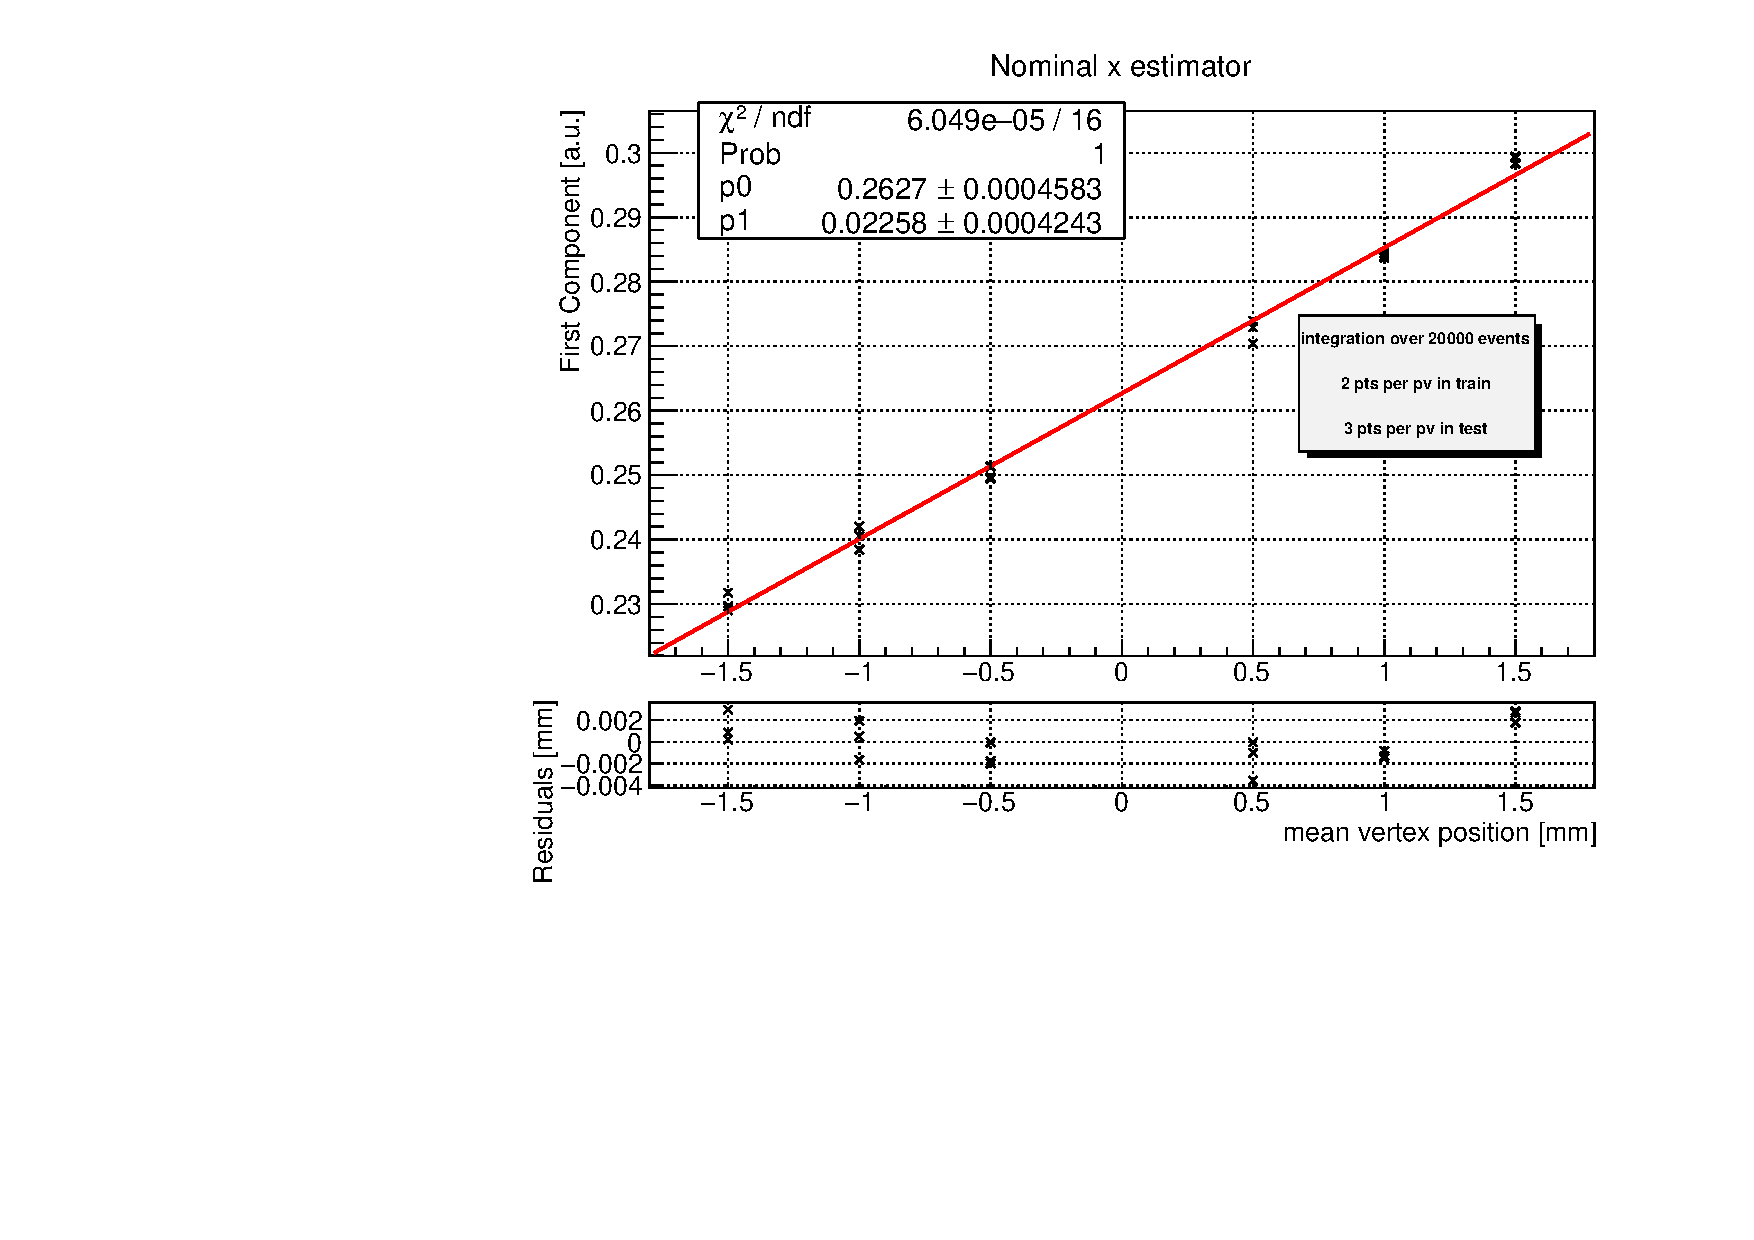
\includegraphics[width=\linewidth]{figures/x_fit_veloA_MC_normalized.pdf}
    \caption{Linear Fit}\label{fig:x_veloA_fit_MC}
    \end{subfigure}
    \begin{subfigure}{0.48\textwidth}
    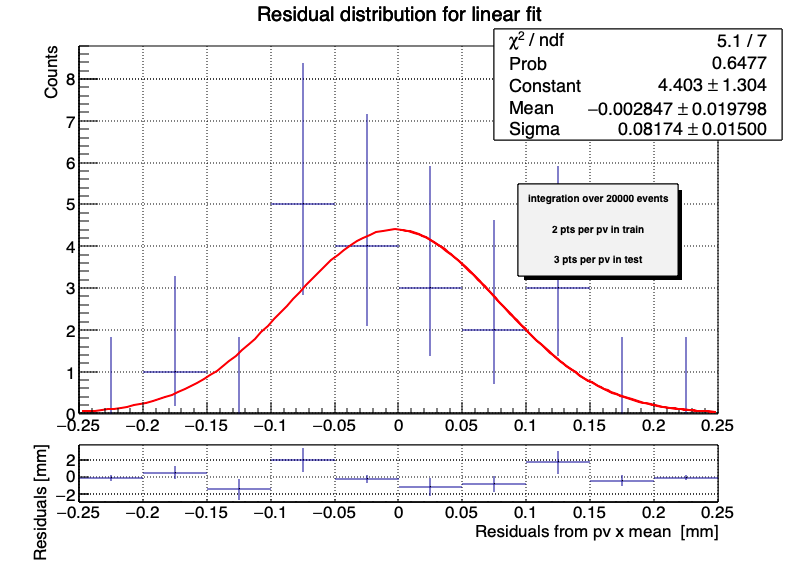
\includegraphics[width=\linewidth]{figures/x_res_veloA_MC.png}
    \caption{Residuals from the fit of the graph on the left. }\label{fig:x_veloA_res_MC}
    \end{subfigure}
    \caption{Linearity of the first component PC (divided by $\mu=5.5$) with respect to virtual VELO A position shifts in x component, alongside the residuals distribution fitted with a Gaussian distribution.}
    \label{fig:x_veloA_MC}
\end{figure}


\begin{figure}
    \centering
    \begin{subfigure}{0.48\textwidth}
    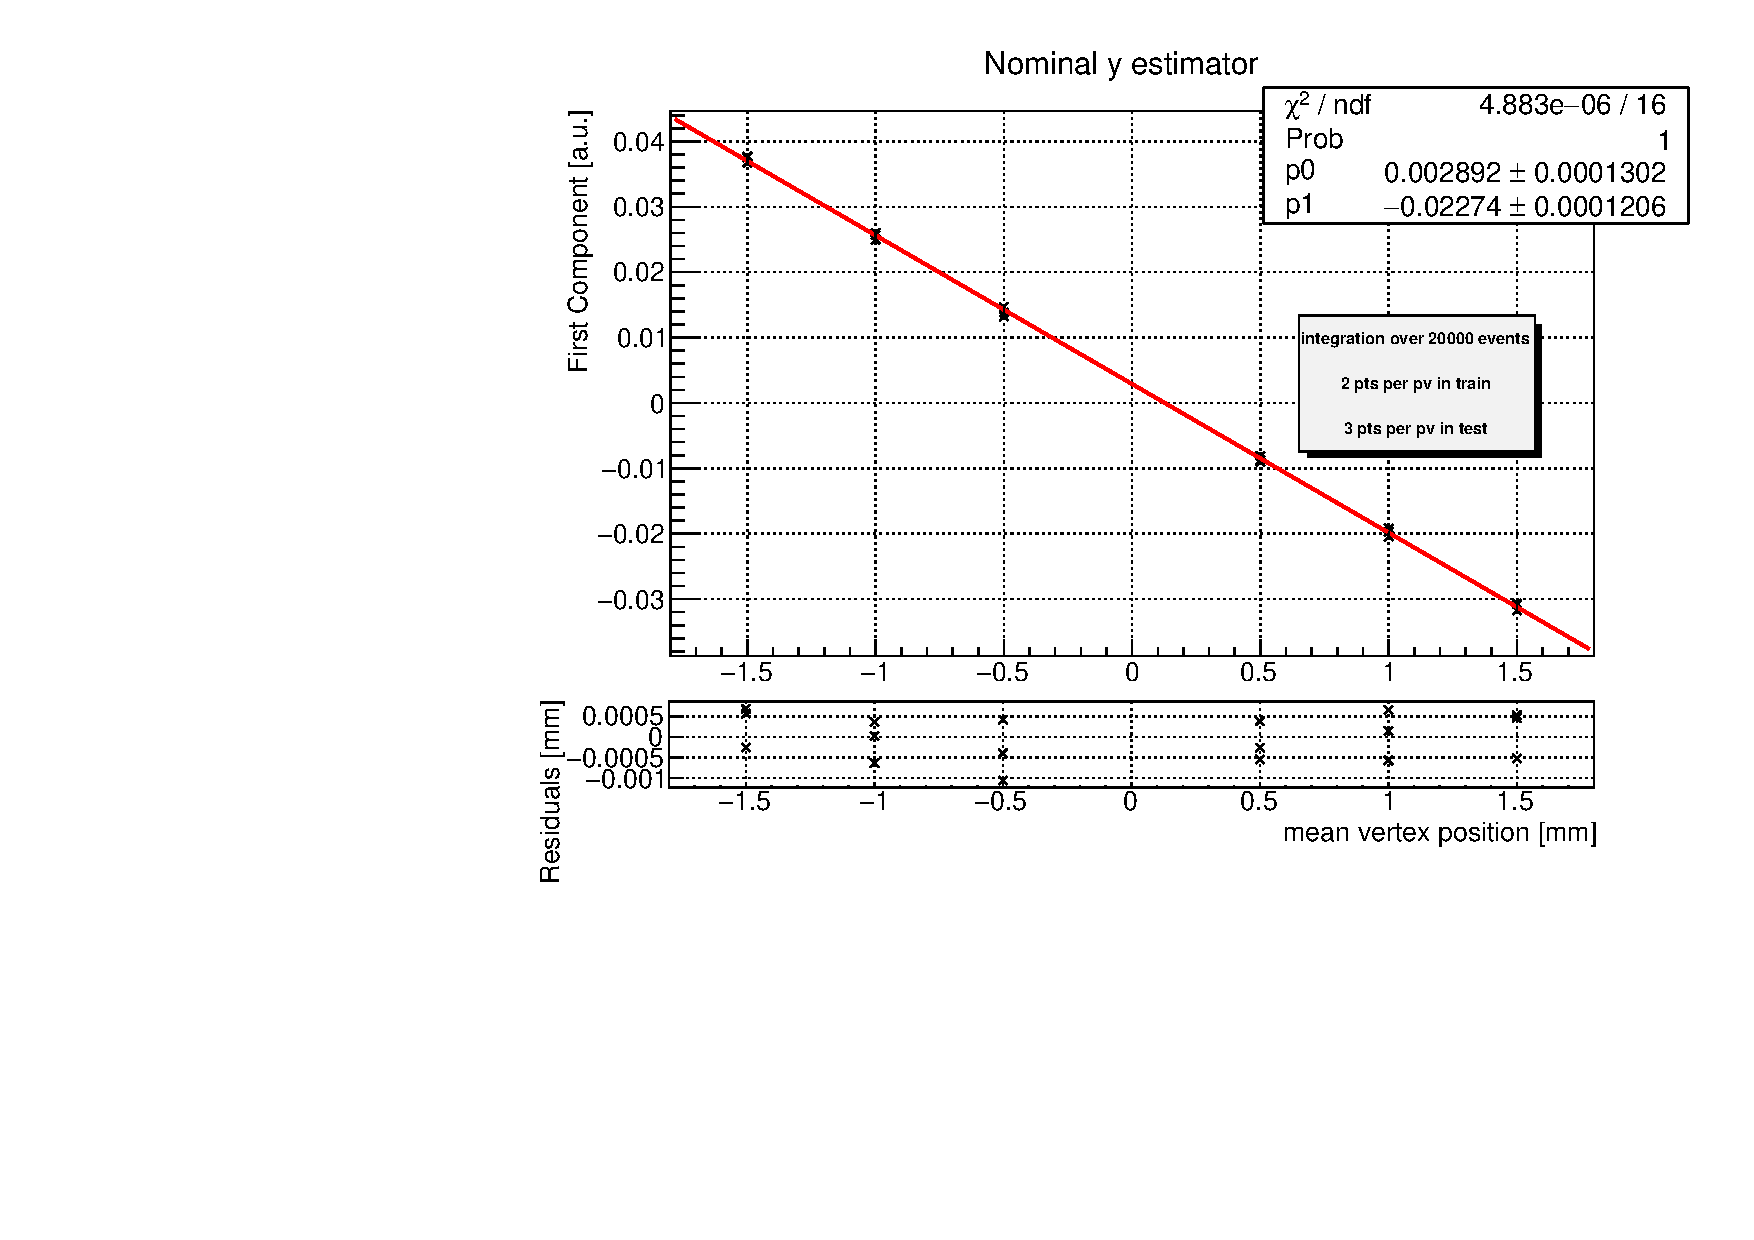
\includegraphics[width=\linewidth]{figures/y_fit_veloA_MC_normalised.pdf}
    \caption{Linear Fit}\label{fig:y_veloA_fit_MC}
    \end{subfigure}
    \begin{subfigure}{0.48\textwidth}
    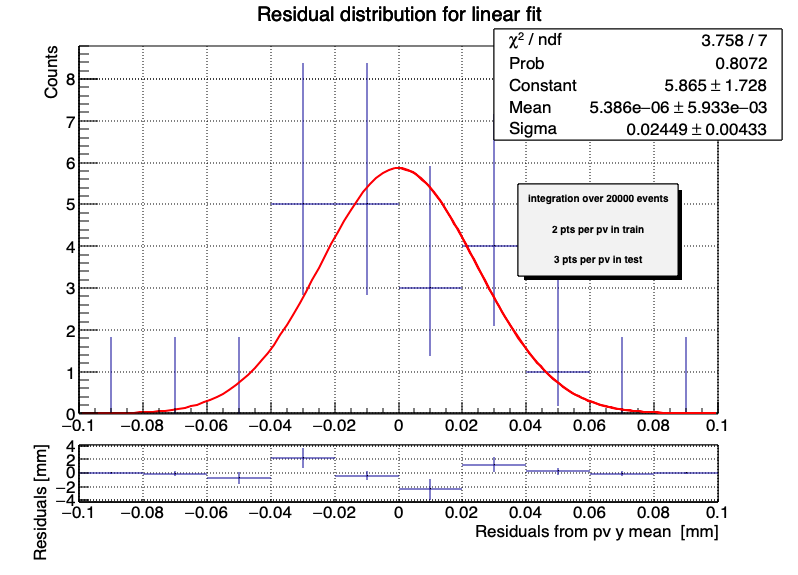
\includegraphics[width=\linewidth]{figures/y_res_veloA_MC.png}
    \caption{Residuals from the fit of the graph on the left. }\label{fig:y_veloA_res_MC}
    \end{subfigure}
    \caption{Linearity of the first PC (divided by $\mu=5.5$) with respect to virtual VELO A position shifts in y component, alongside the residuals distribution fitted with a Gaussian distribution.}
    \label{fig:y_veloA_MC}
\end{figure}

\begin{figure}
    \centering
    \begin{subfigure}{0.48\textwidth}
    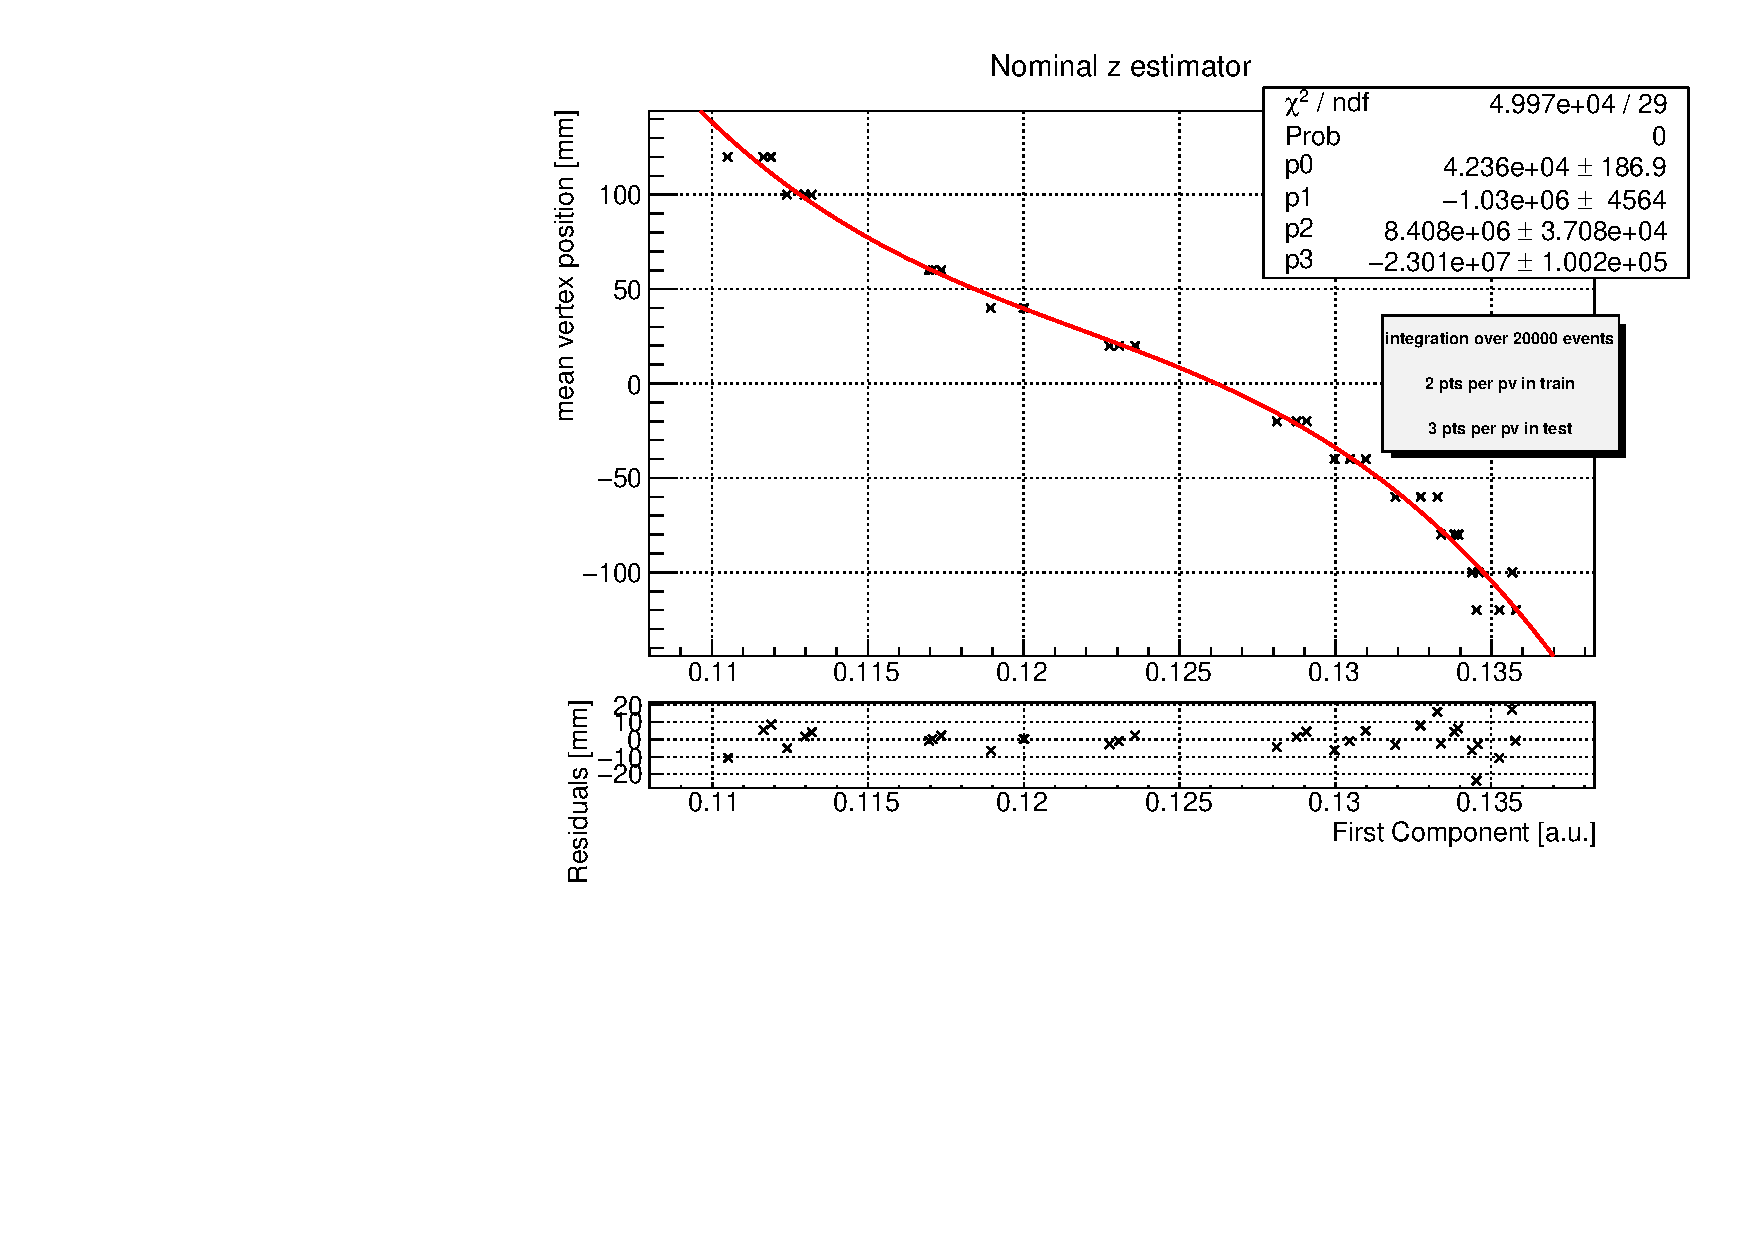
\includegraphics[width=\linewidth]{figures/z_fit_veloA_normalised.pdf}
    \caption{Cubic Fit}\label{fig:z_veloA_fit_MC}
    \end{subfigure}
    \begin{subfigure}{0.48\textwidth}
    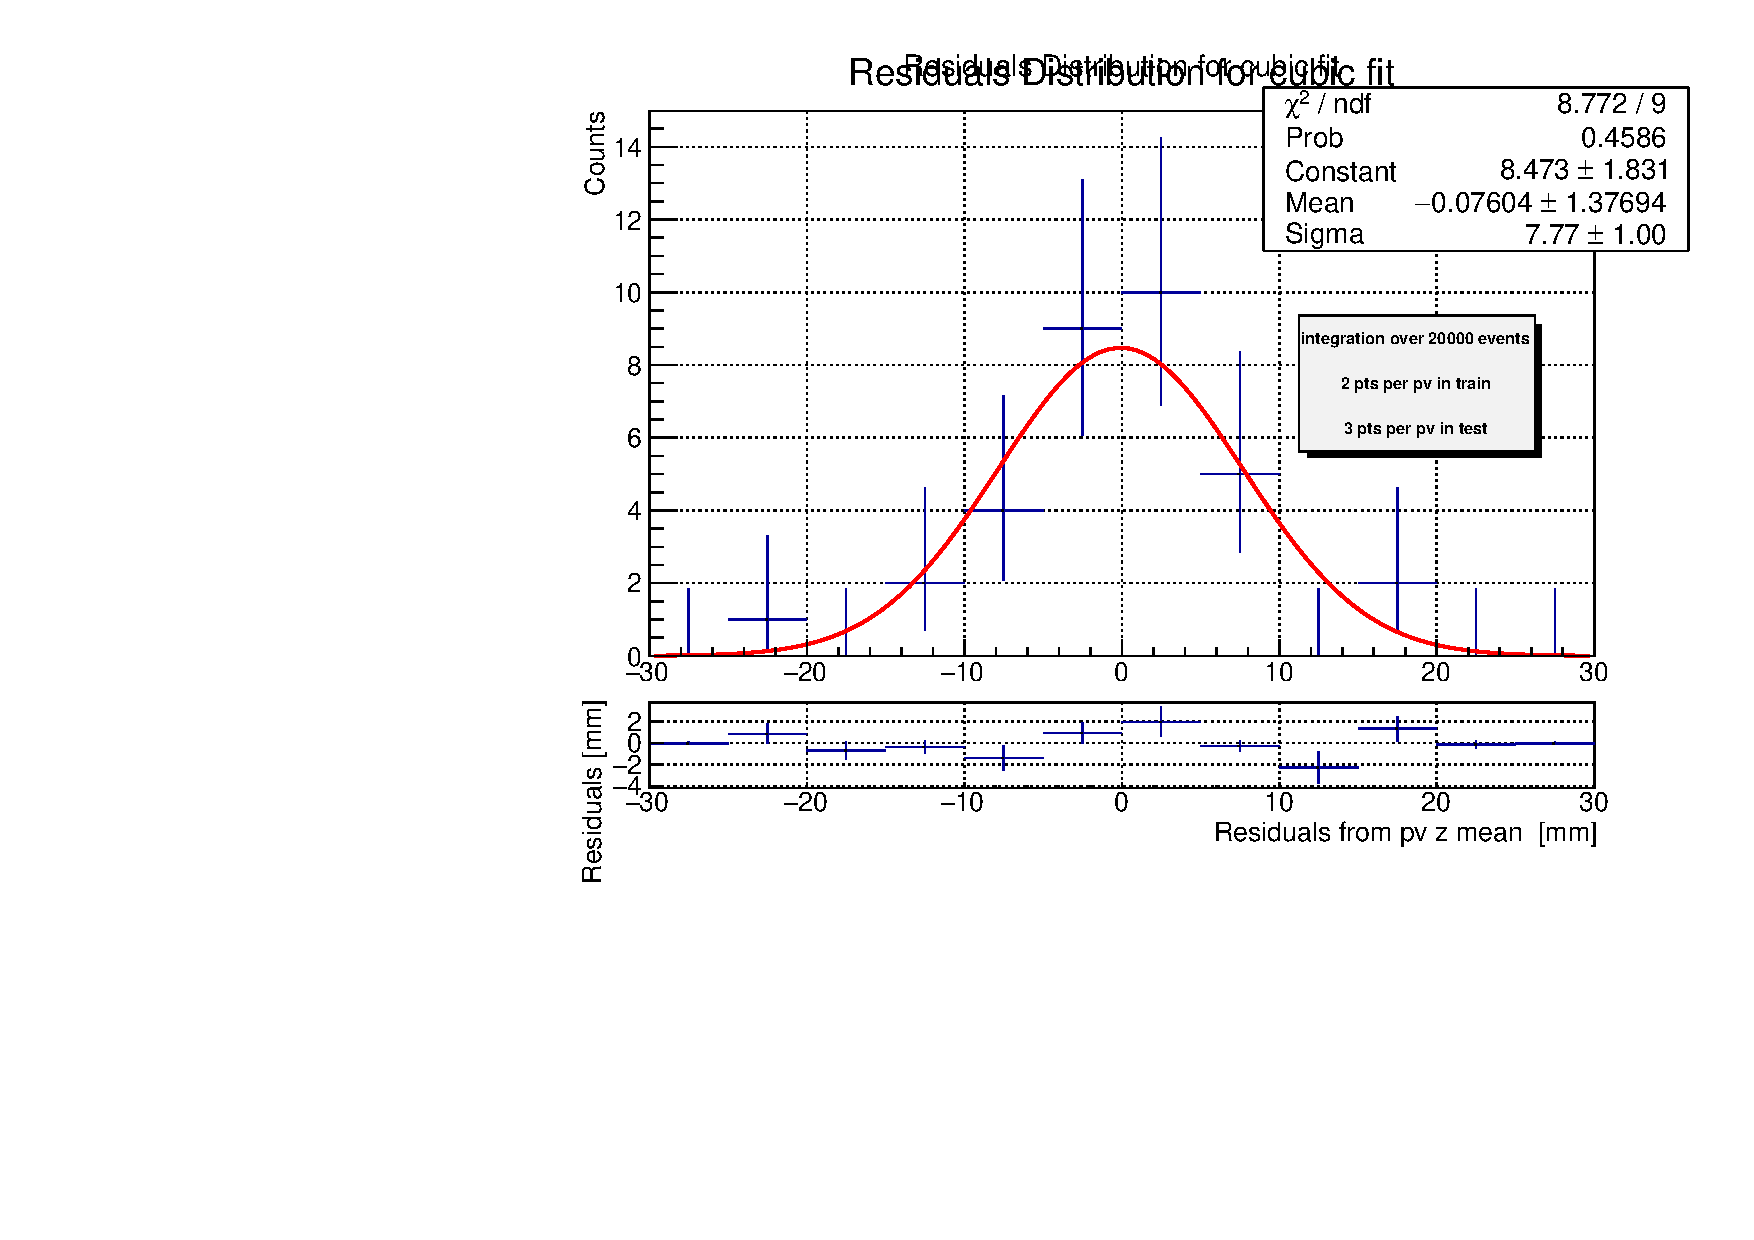
\includegraphics[width=\linewidth]{figures/z_res_veloA_normalised.pdf}
    \caption{Residuals from the fit of the graph on the left. }\label{fig:z_veloA_res_MC}
    \end{subfigure}
    \caption{Cubic relationship of the first PC (divided by $\mu=5.5$) with the PCA with respect to virtual VELO A position shifts in z component, alongside the residuals distribution fitted with a Gaussian distribution.}
    \label{fig:z_veloA_MC}
\end{figure}

\begin{figure}
    \centering
    \begin{subfigure}{0.48\textwidth}
    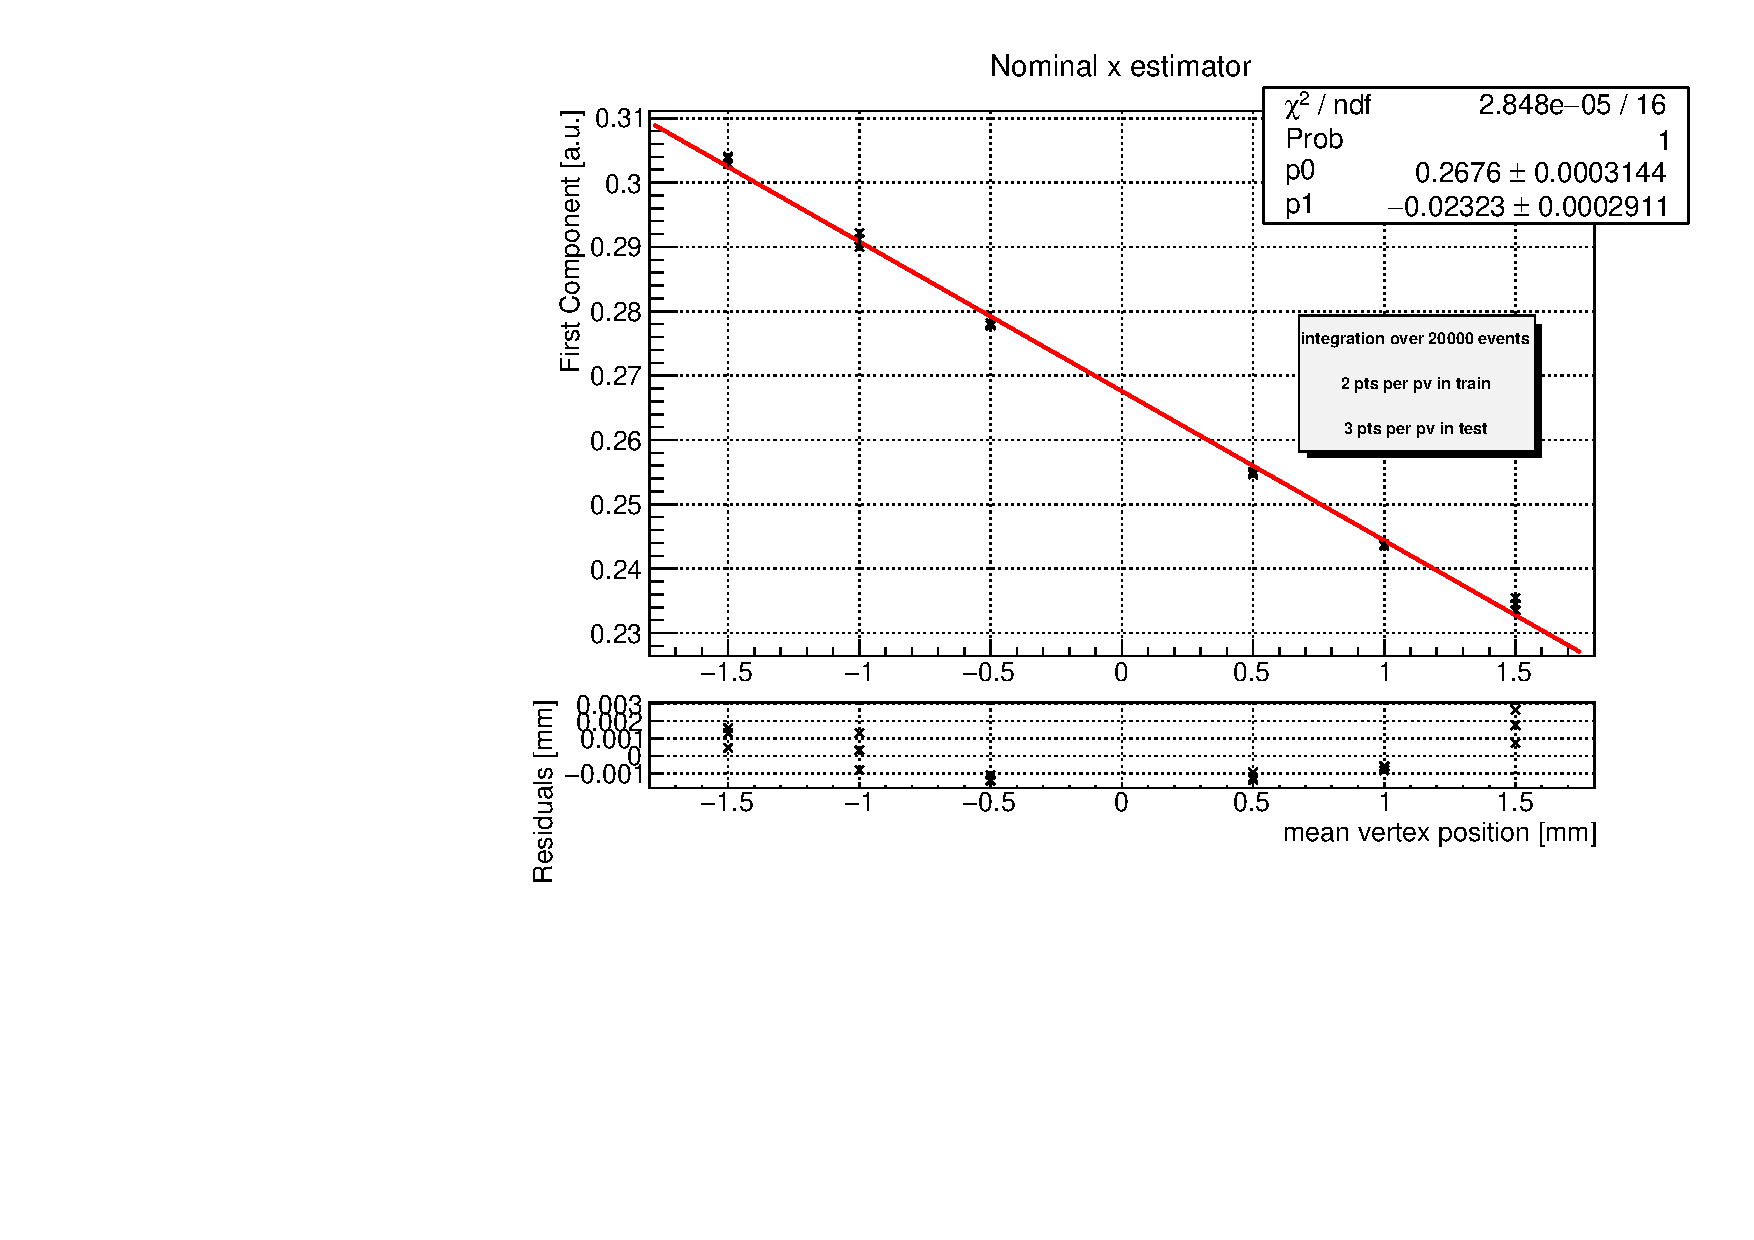
\includegraphics[width=\linewidth]{figures/x_fit_veloC_MC_normalised.pdf}
    \caption{Linear Fit}\label{fig:x_veloC_fit_MC}
    \end{subfigure}
    \begin{subfigure}{0.48\textwidth}
    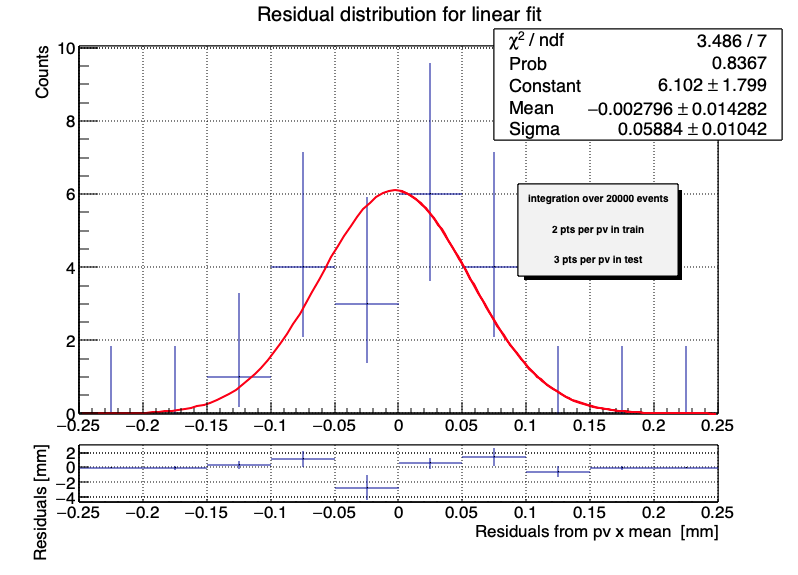
\includegraphics[width=\linewidth]{figures/x_res_veloC_MC.png}
    \caption{Residuals from the fit of the graph on the left. }\label{fig:x_veloC_res_MC}
    \end{subfigure}
    \caption{Linearity of the first PC (divided by $\mu=5.5$) with respect to  virtual VELO C position shifts in x component, alongside the residuals distribution fitted with a Gaussian distribution.}
    \label{fig:x_veloC_MC}
\end{figure}
\begin{figure}
    \centering
    \begin{subfigure}{0.48\textwidth}
    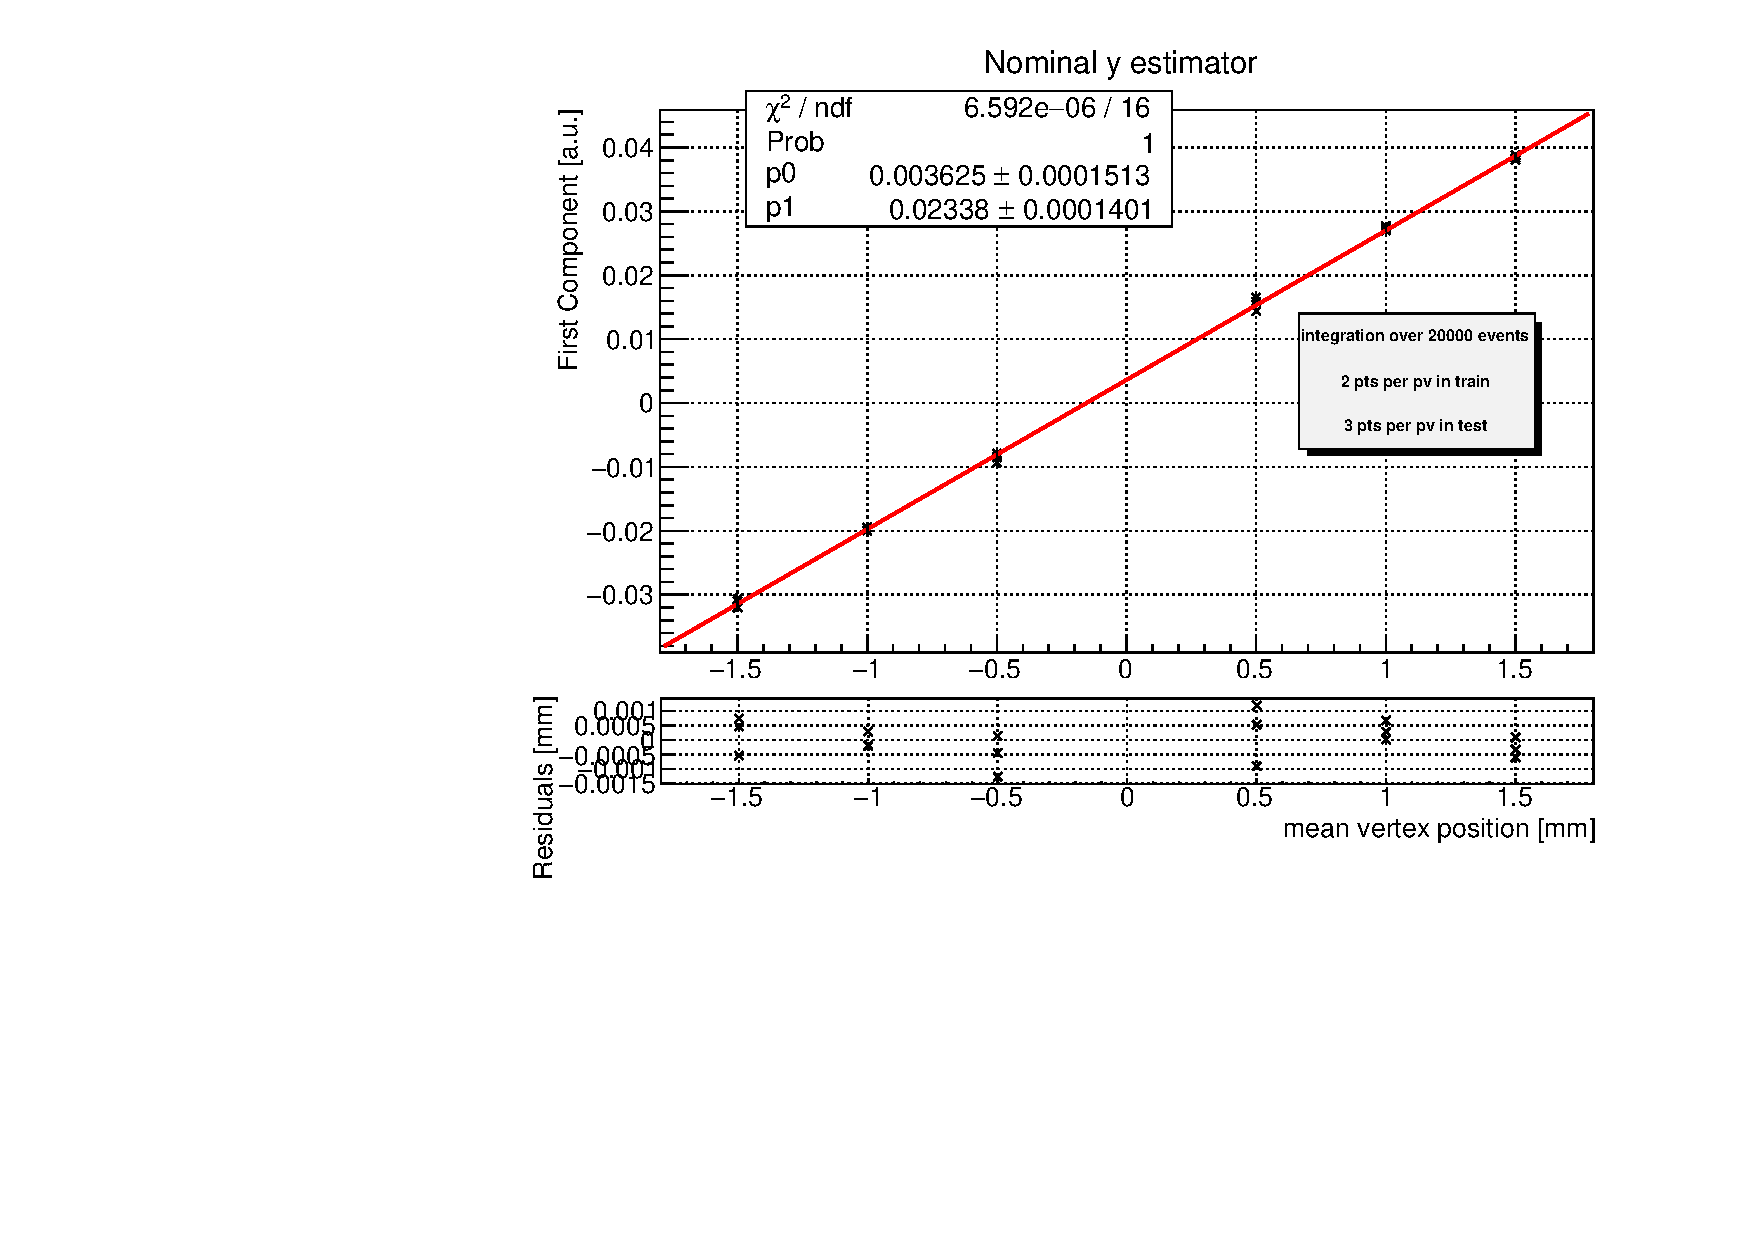
\includegraphics[width=\linewidth]{figures/y_fit_veloC_MC_normalised.pdf}
    \caption{Linear Fit}\label{fig:y_veloC_fit_MC}
    \end{subfigure}
    \begin{subfigure}{0.48\textwidth}
    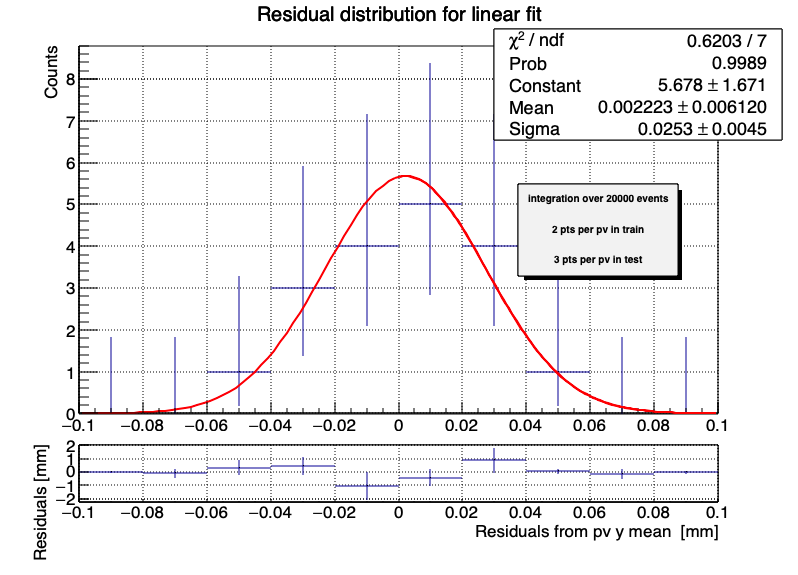
\includegraphics[width=\linewidth]{figures/y_res_veloC_MC.png}
    \caption{Residuals from the fit of the graph on the left. }\label{fig:y_veloC_res_MC}
    \end{subfigure}
    \caption{Linearity of the first PC (divided by $\mu=5.5$) with respect to  virtual VELO C position shifts in y component, alongside the residuals distribution fitted with a Gaussian distribution.}
    \label{fig:y_veloC_MC}
\end{figure}

\begin{figure}
    \centering
    \begin{subfigure}{0.48\textwidth}
    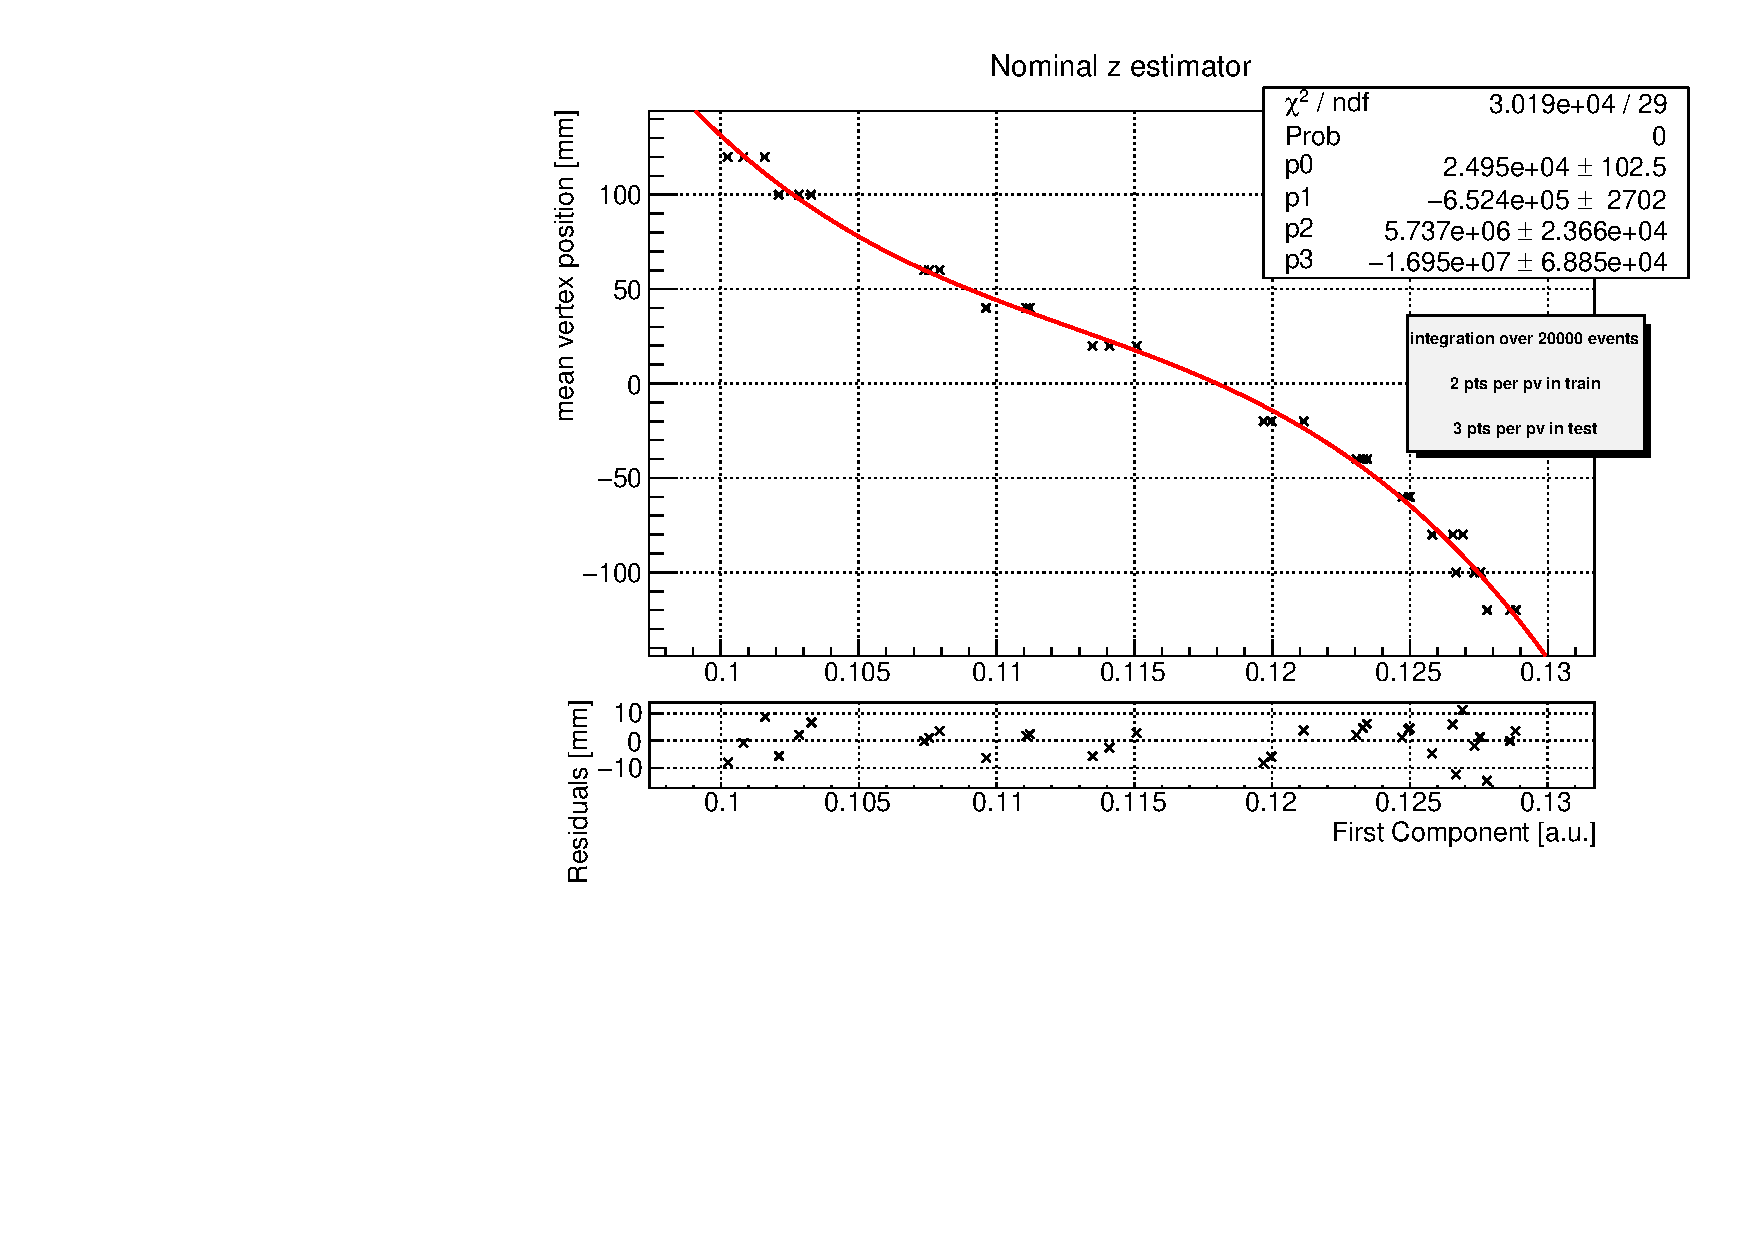
\includegraphics[width=\linewidth]{figures/z_fit_veloC_MC_residuals.pdf}
    \caption{Cubic Fit}\label{fig:z_veloC_fit_MC}
    \end{subfigure}
    \begin{subfigure}{0.48\textwidth}
    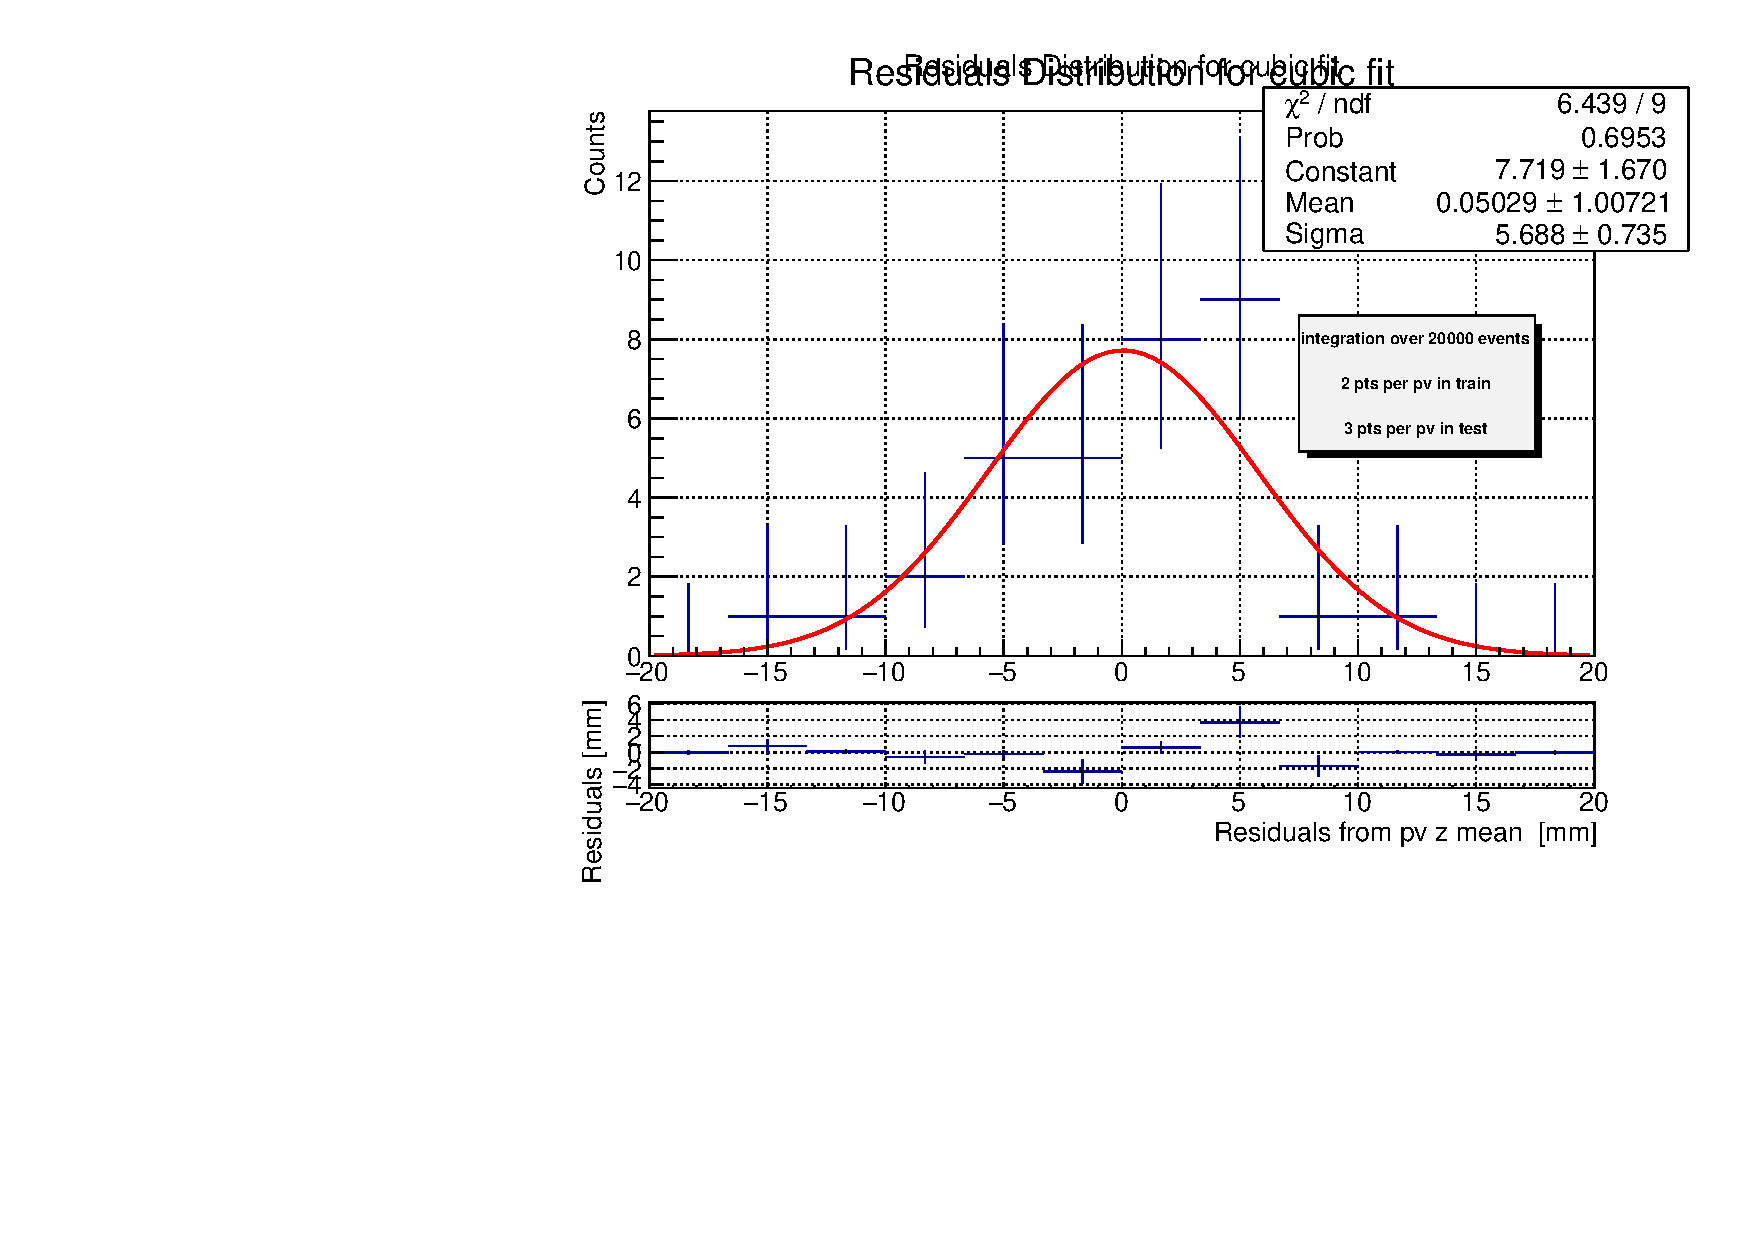
\includegraphics[width=\linewidth]{figures/z_res_veloC_MC_normalised.pdf}
    \caption{Residuals from the fit of the graph on the left. }\label{fig:z_veloC_res_MC}
    \end{subfigure}
    \caption{Cubic relationship between the first PC (divided by $\mu=5.5$) with respect to virtual VELO C position shifts in the z component, alongside the residuals distribution fitted with a Gaussian distribution.}
    \label{fig:z_veloC_MC}
\end{figure}

For both halves there still is a linear relation between the scores and the VELO positions in the $x$ and $y$ component, while the relation remains cubic for the $z$ scores.  Furthermore, the standard deviation estimated from the Gaussian fitted in the residuals histogram of Figures \ref{fig:x_veloA_res_MC}, \ref{fig:y_veloA_res_MC}, \ref{fig:z_veloA_res_MC}, \ref{fig:x_veloC_res_MC}, \ref{fig:y_veloC_res_MC}, \ref{fig:z_veloC_res_MC} yields a resolution between \SI{25}{\micro\meter} and \SI{81}{\micro\meter} for the transverse components $x$ and $y$, while for the $z$ component the value is around \SI{7}{\milli\meter}. As in the previous chapter, we expect the resolution for the $z$ component to be worse than the ones of the variables in the transverse plane to the beamline. Furthermore, these resolutions quoted here were obtained integrating 20000 events, i.e. computing an estimate every \SI{870}{\micro\second} at $\mu=5.5$.

Since the relation is essentially of the same form of equation~\eqref{x_hat_corrected}, we can estimate the various coefficients from the fit performed in the scatter plots \ref{fig:x_veloA_fit_MC}, \ref{fig:y_veloA_fit_MC}, \ref{fig:z_veloA_fit_MC}, \ref{fig:x_veloC_fit_MC}, \ref{fig:y_veloC_fit_MC}, \ref{fig:z_veloC_fit_MC}. Regarding the $z$ variable, the coefficients obtained are directly those plotted in the canvas. For the $x$ and $y$ components, we have to invert the relationship. In fact
\begin{equation}
    y = p_1\cdot x +p_0 \quad  \Longrightarrow \quad  x = \frac{y}{p_1}-\frac{p_0}{p_1},
\end{equation}
meaning that the coefficients of equations \eqref{x_hat_corrected} need to be computed as 
\begin{equation}
    a = \frac{1}{p_1} \qquad b = -\frac{p_0}{p_1}.
\end{equation}
We can therefore write the estimator for each side $s$=A,C with equation \eqref{eq:velo_hat}, using the coefficients reported in Table~\ref{tab:coefficients}.
\begin{equation}
\begin{split}
    \hat{x}^{s} &= a_x^s \frac{t^x_1}{\mu} + b_x^s\\%\qquad
    \hat{y}^{s} &=a_y^s \frac{t^y_1}{\mu} + b_y^s \\%\qquad
    \hat{z}^{s} &=a_z^s\biggl(\frac{t^z_1}{\mu}\biggr)^3 + b_z^s\biggl(\frac{t^z_1}{\mu}\biggr)^2 + c_z^s \frac{t^z_1}{\mu} + d^s
    \end{split} \label{eq:velo_hat}
    \end{equation}
    
\begin{table}
\centering
\begin{tabular}{c|c|c|c|c|c|c}
coefficient  & $x_A$   & $y_A$   & $z_A$      & $x_C$   & $y_C$  & $z_C$      \\\hline
a & $44.29$  & $-43.97$ &  $-23008090$    & $-43.05$ & $42.77$ &   $-16950459$   \\
b & $-11.63$ & $0.1272$ & $8408082$   & $11.99$  & $-0.15$ &  $5736989$ \\
c &        &        & $-103031$   &        &       &  $-652426 $  \\
d &        &        &  $42358$ &        &       & $24954$
\end{tabular}
\caption{Summary of the coefficients for each estimator in the form of equation \eqref{eq:velo_hat}}\label{tab:coefficients}
\end{table}

\section{Calibration on real data}
We can perform another calibration for the $x$ and $y$ estimators of both VELO halves by directly relying on real collision data, using the same LSC performed on April 6th, 2024. 
Once again, we perform the exercise of considering the luminous region as fixed in space and the VELO moving with respect to this reference. By doing so, we can use the same LSC scans that were used to calibrate the luminous region estimators in the previous chapter. For the comparison, we rely on the reconstructed position of the VELO halves provided by the monitoring tasks of the VELO system, that reads a subset of minimum bias events at \SI{30}{\kilo\hertz}. 

\begin{figure}
    \centering
    \begin{subfigure}{0.48\textwidth}
    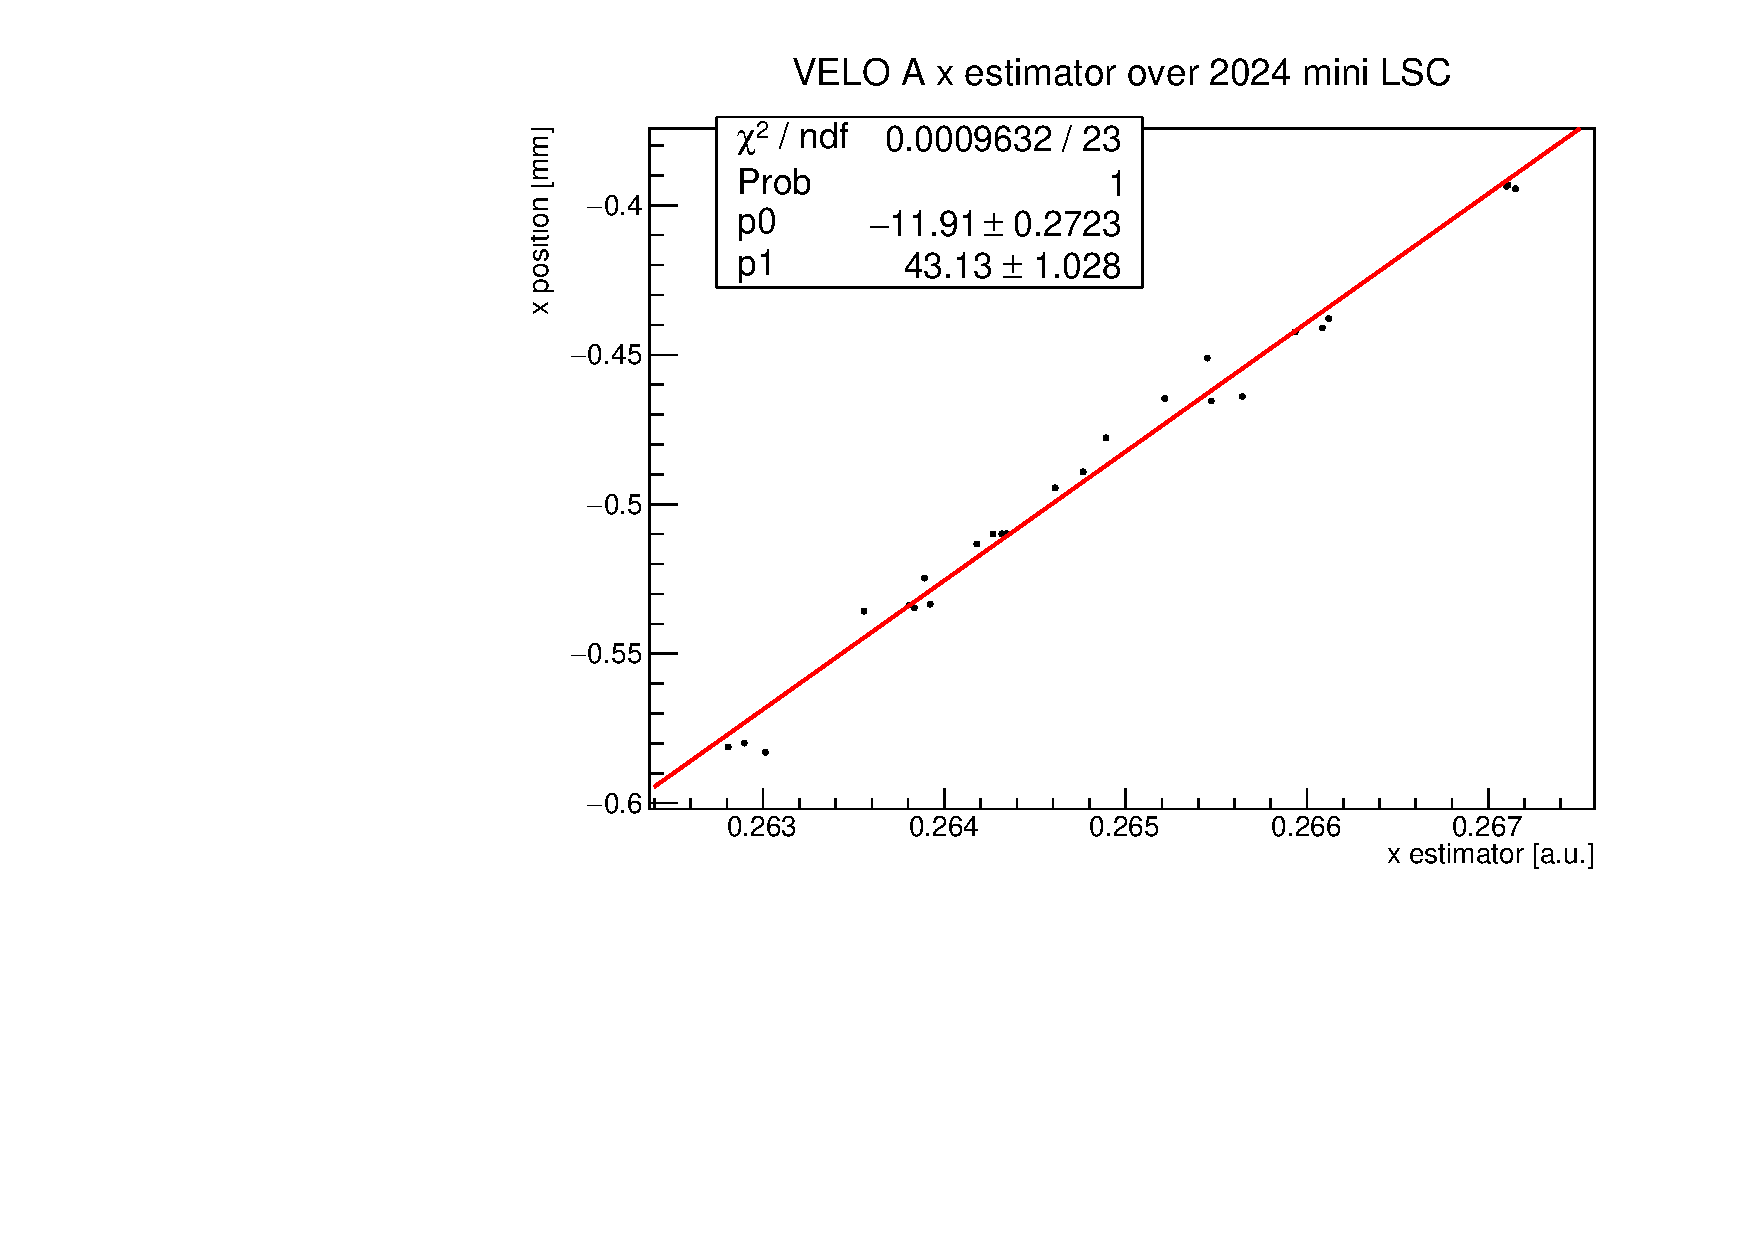
\includegraphics[width=\linewidth]{figures/x_fit_VELO_A_data.pdf}
    \caption{Linear Fit}\label{fig:x_veloA_fit_data}
    \end{subfigure}
    \begin{subfigure}{0.48\textwidth}
    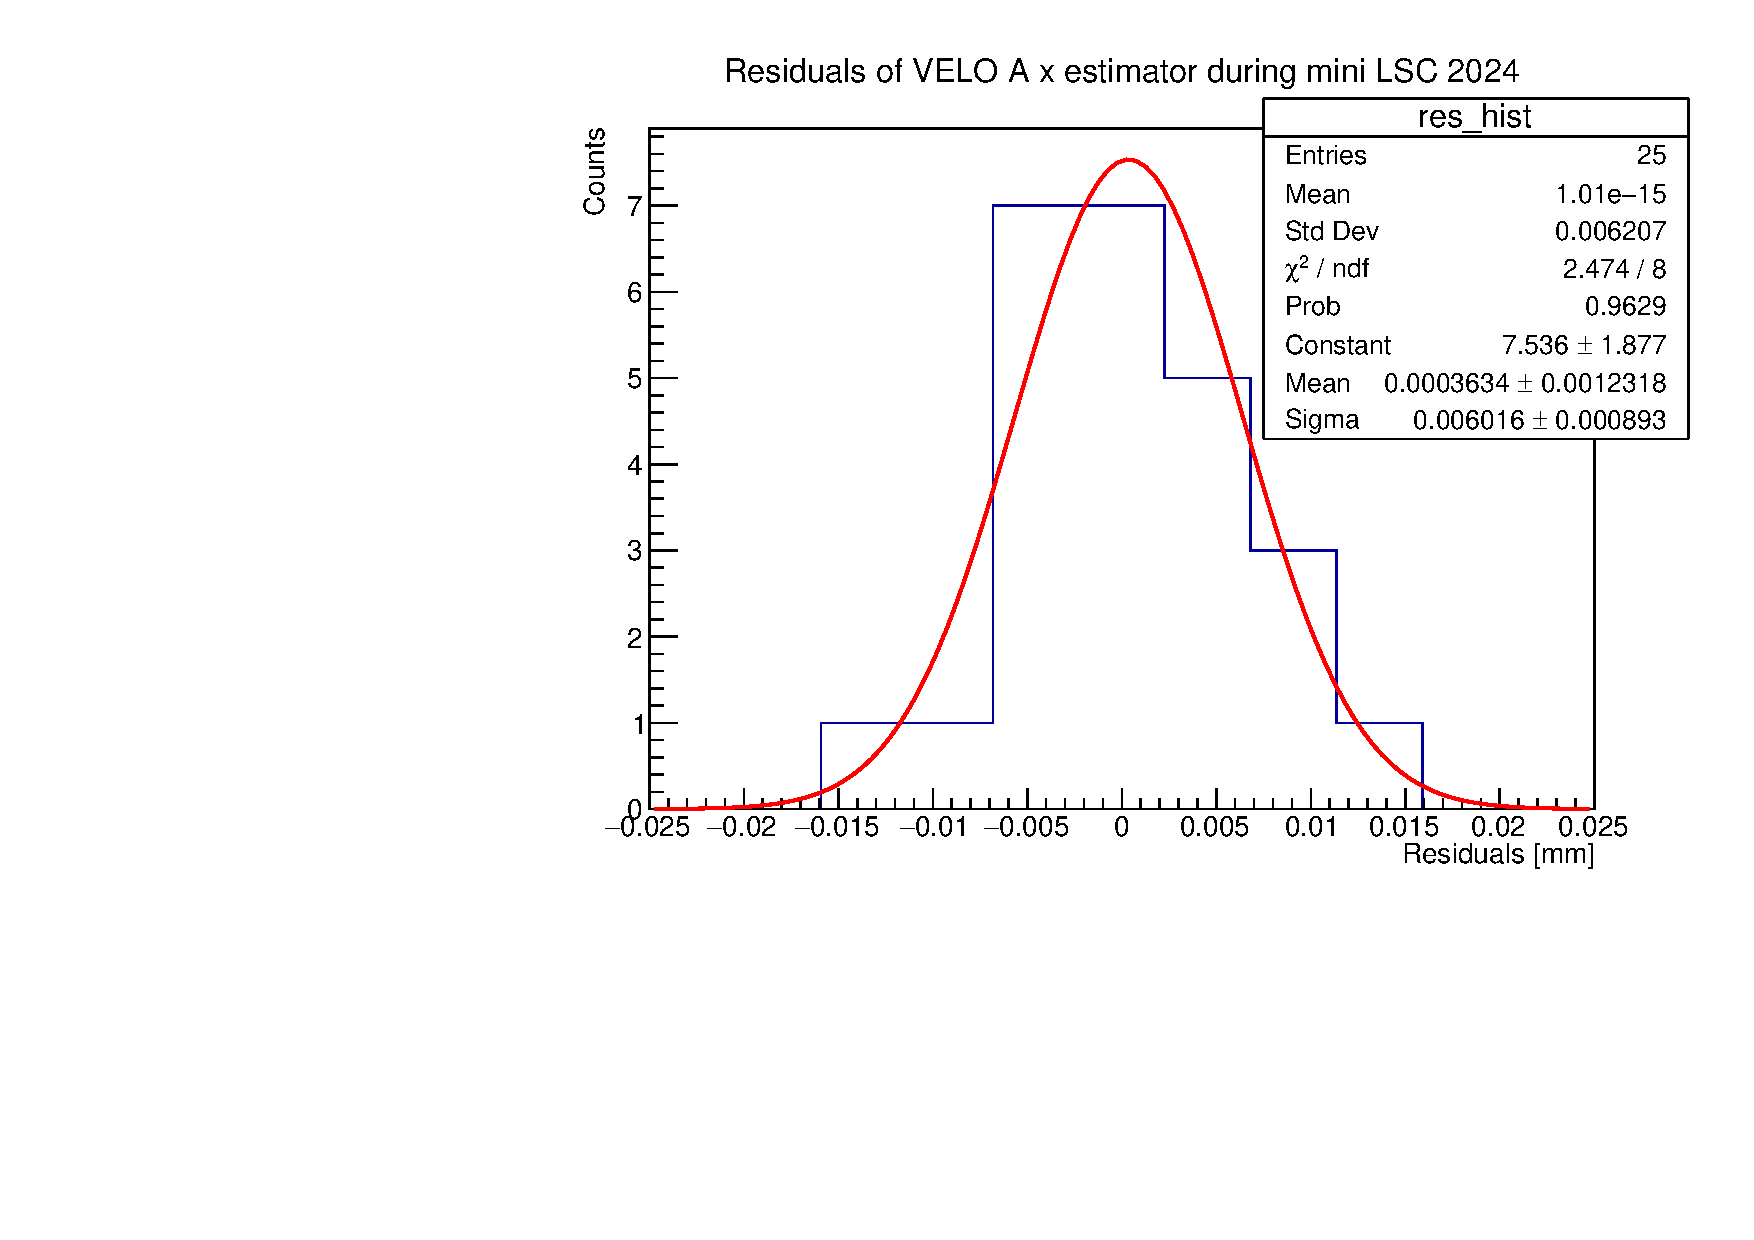
\includegraphics[width=\linewidth]{figures/x_res_VELO_A_data.pdf}
    \caption{Residuals from the fit of the graph on the left. }\label{fig:x_veloA_res_data}
    \end{subfigure}
    \caption{Linearity of the first component calculated with the PCA with respect to virtual VELO A position shifts in $x$ component, alongside the residuals distribution fitted with a Gaussian probability density function.}
    \label{fig:x_veloA_data}
\end{figure}


\begin{figure}
    \centering
    \begin{subfigure}{0.48\textwidth}
    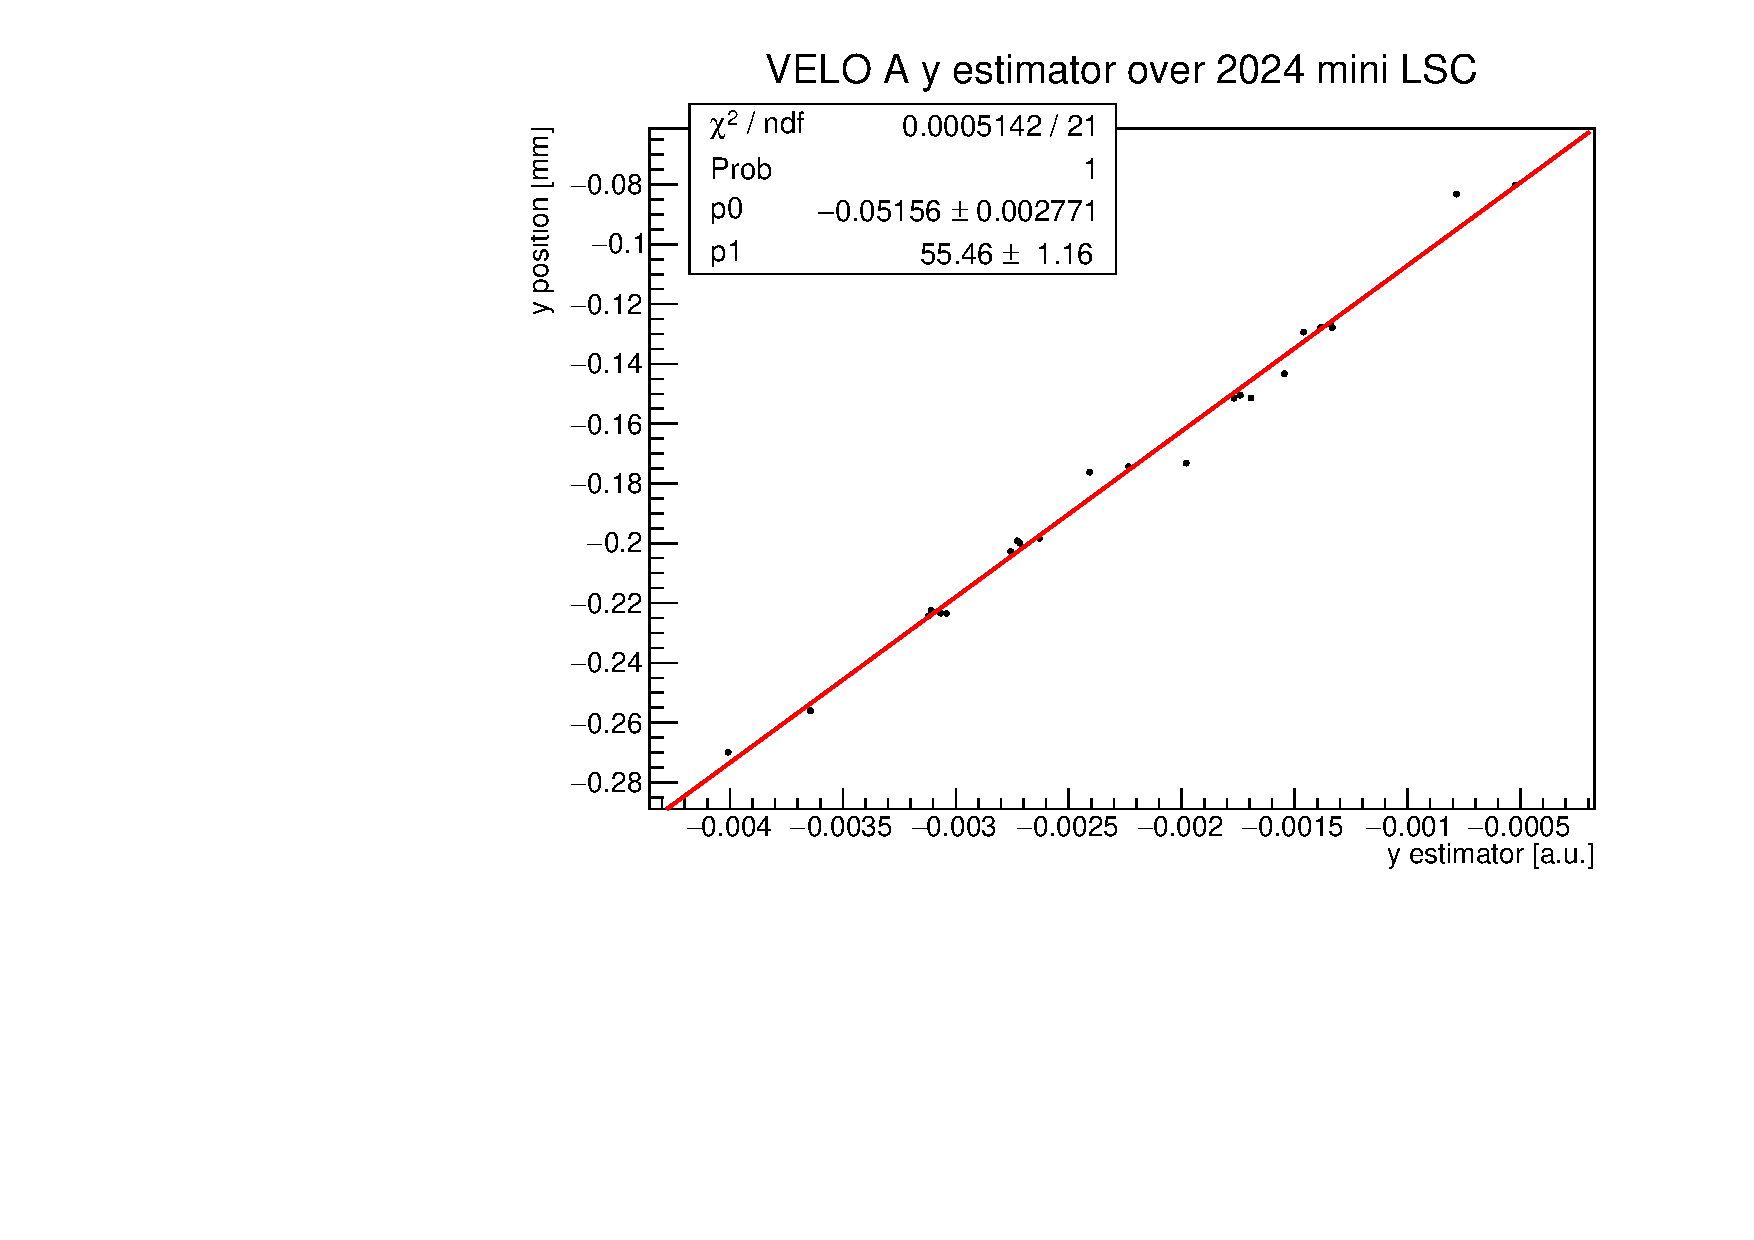
\includegraphics[width=\linewidth]{figures/y_fit_VELO_A_data.pdf}
    \caption{Linear Fit}\label{fig:y_veloA_fit_data}
    \end{subfigure}
    \begin{subfigure}{0.48\textwidth}
    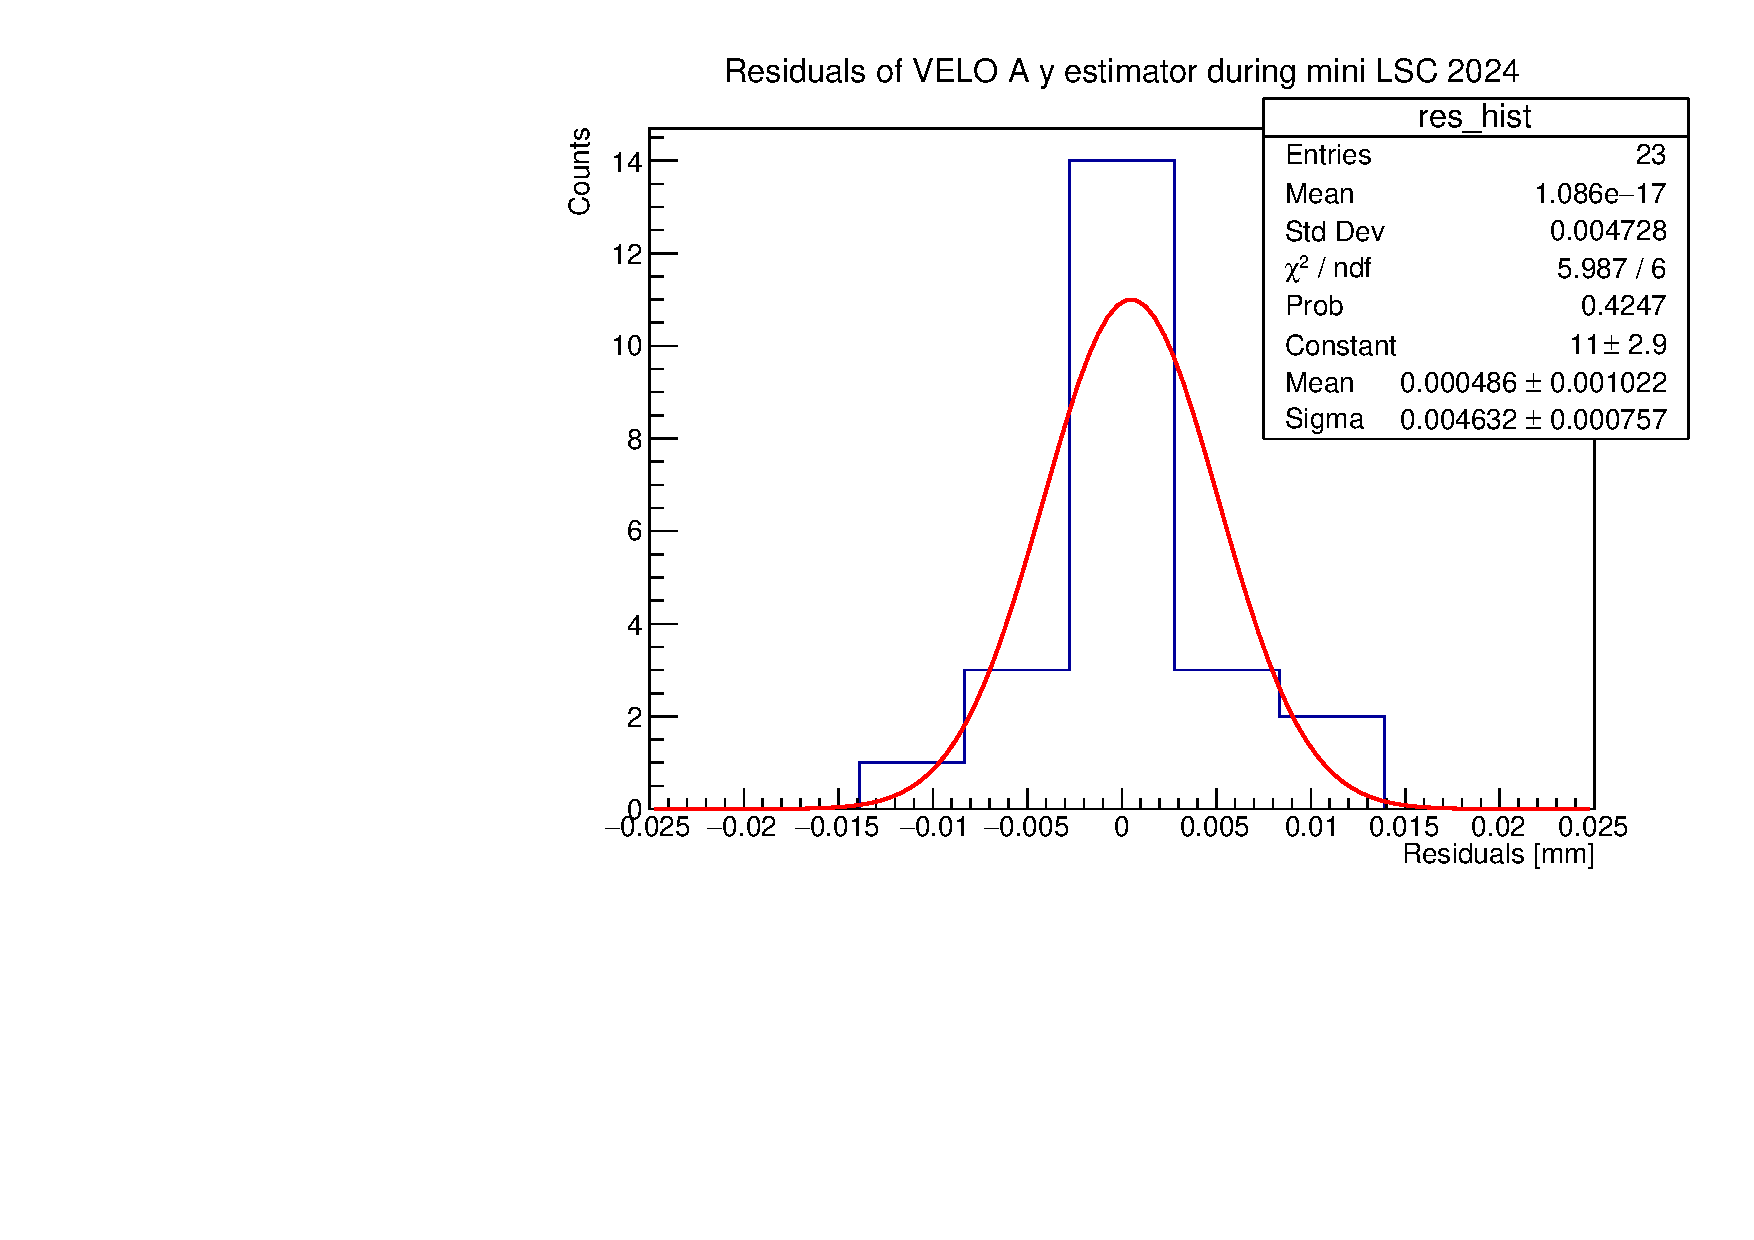
\includegraphics[width=\linewidth]{figures/y_res_VELO_A_data.pdf}
    \caption{Residuals from the fit of the graph on the left. }\label{fig:y_veloA_res_data}
    \end{subfigure}
    \caption{Linearity of the first component calculated with the PCA with respect to virtual VELO A position shifts in $y$ component, alongside the residuals distribution fitted with a Gaussian probability density function.}
    \label{fig:y_veloA_data}
\end{figure}



\begin{figure}
    \centering
    \begin{subfigure}{0.48\textwidth}
    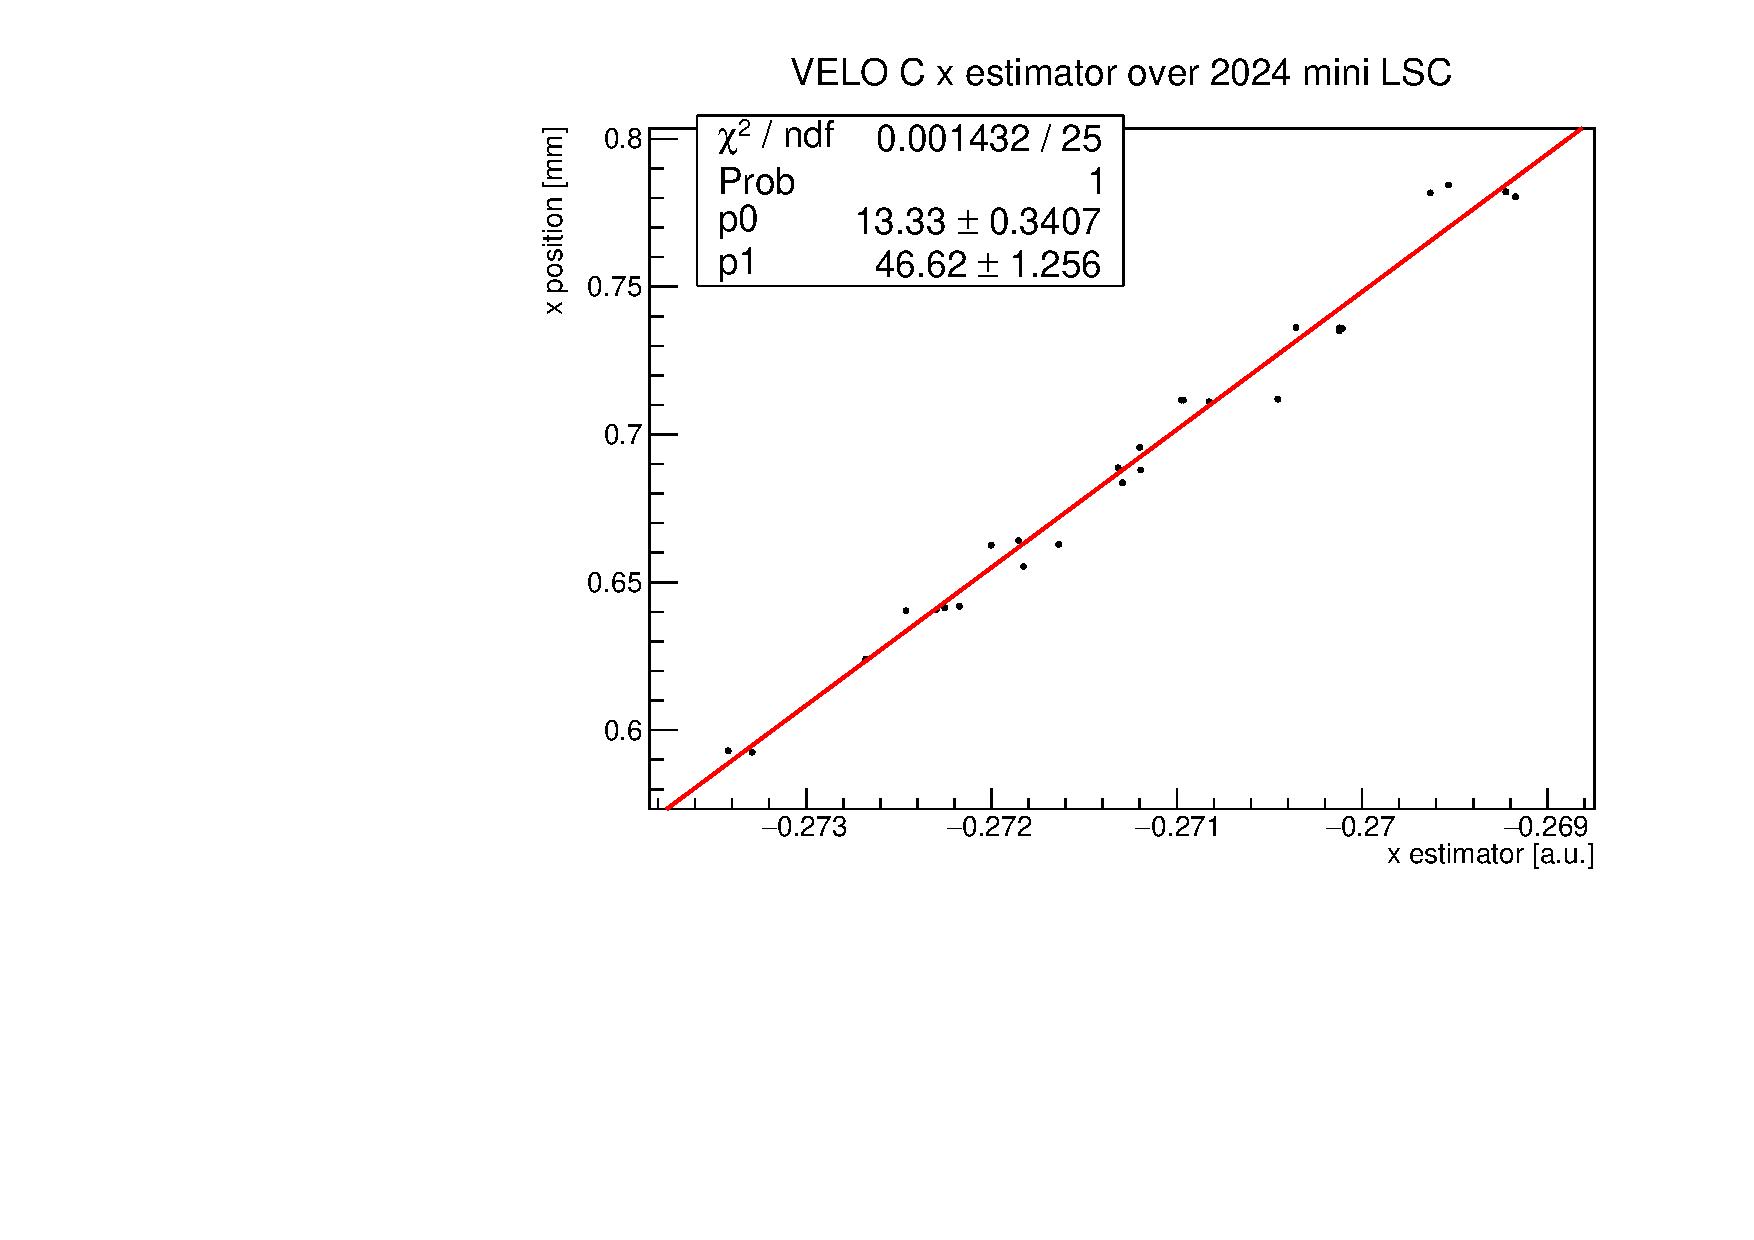
\includegraphics[width=\linewidth]{figures/x_fit_VELO_C_data.pdf}
    \caption{Linear Fit}\label{fig:x_veloC_fit_data}
    \end{subfigure}
    \begin{subfigure}{0.48\textwidth}
    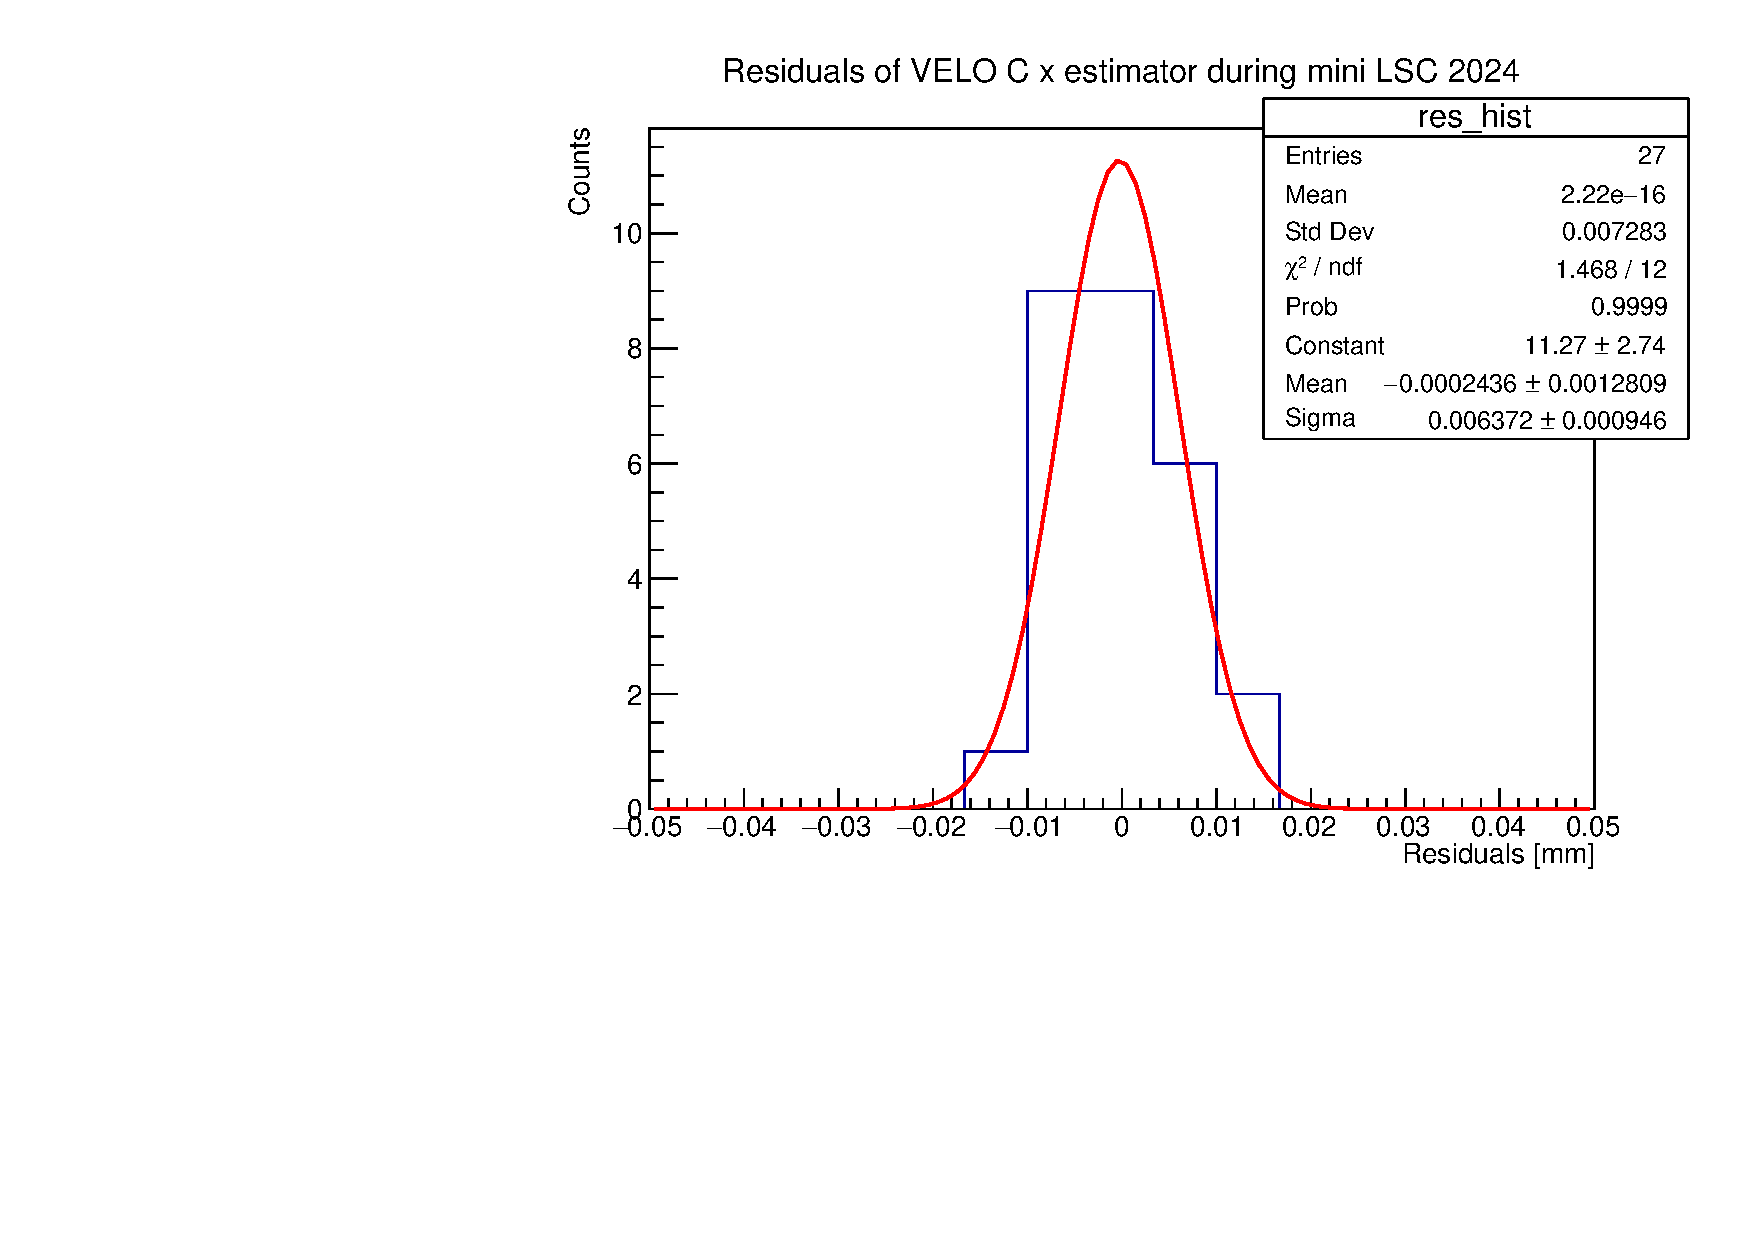
\includegraphics[width=\linewidth]{figures/x_res_VELO_C_data.pdf}
    \caption{Residuals from the fit of the graph on the left. }\label{fig:x_veloC_res_data}
    \end{subfigure}
    \caption{Linearity of the first component calculated with the PCA with respect to  virtual VELO C position shifts in $x$ component, alongside the residuals distribution fitted with a Gaussian probability density function.}
    \label{fig:x_veloC_data}
\end{figure}
\begin{figure}
    \centering
    \begin{subfigure}{0.48\textwidth}
    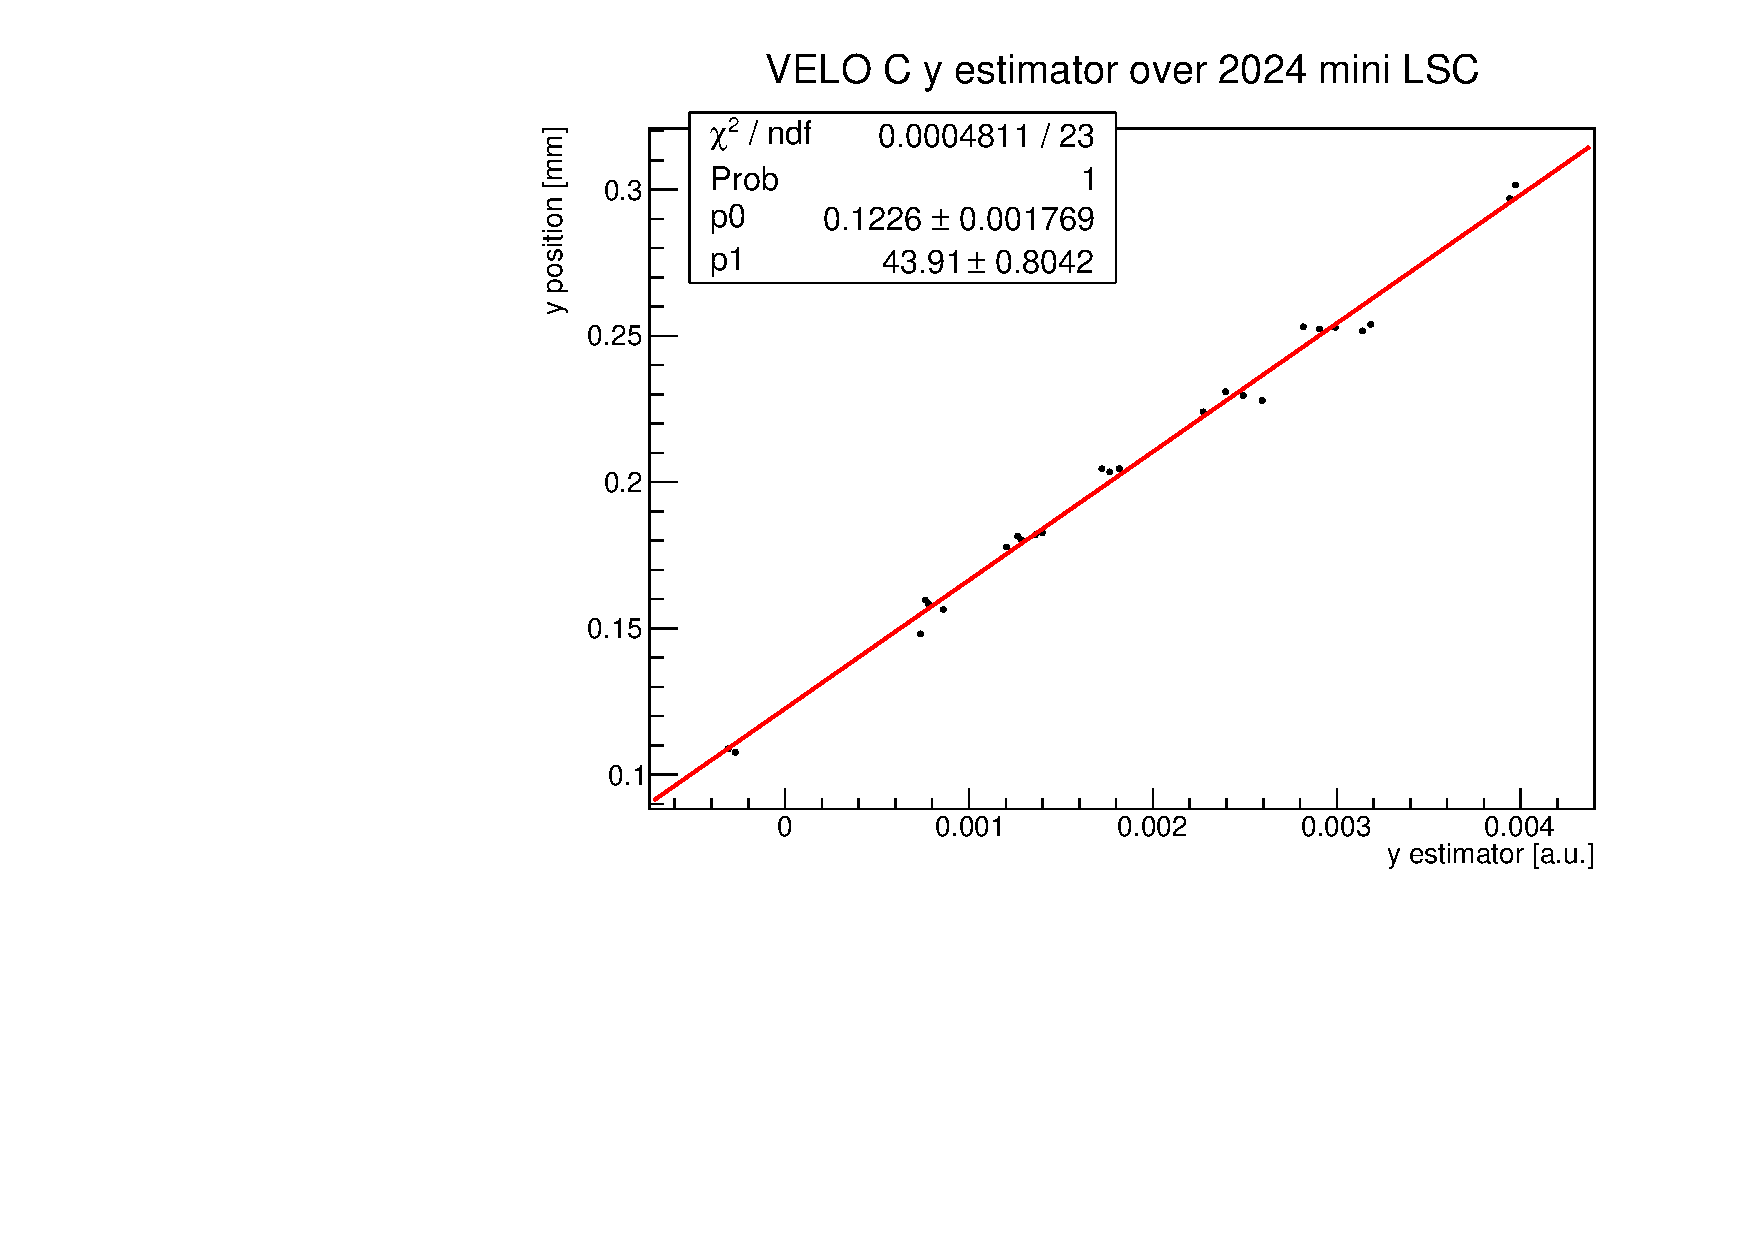
\includegraphics[width=\linewidth]{figures/y_fit_VELO_C_data.pdf}
    \caption{Linear Fit}\label{fig:y_veloC_fit_data}
    \end{subfigure}
    \begin{subfigure}{0.48\textwidth}
    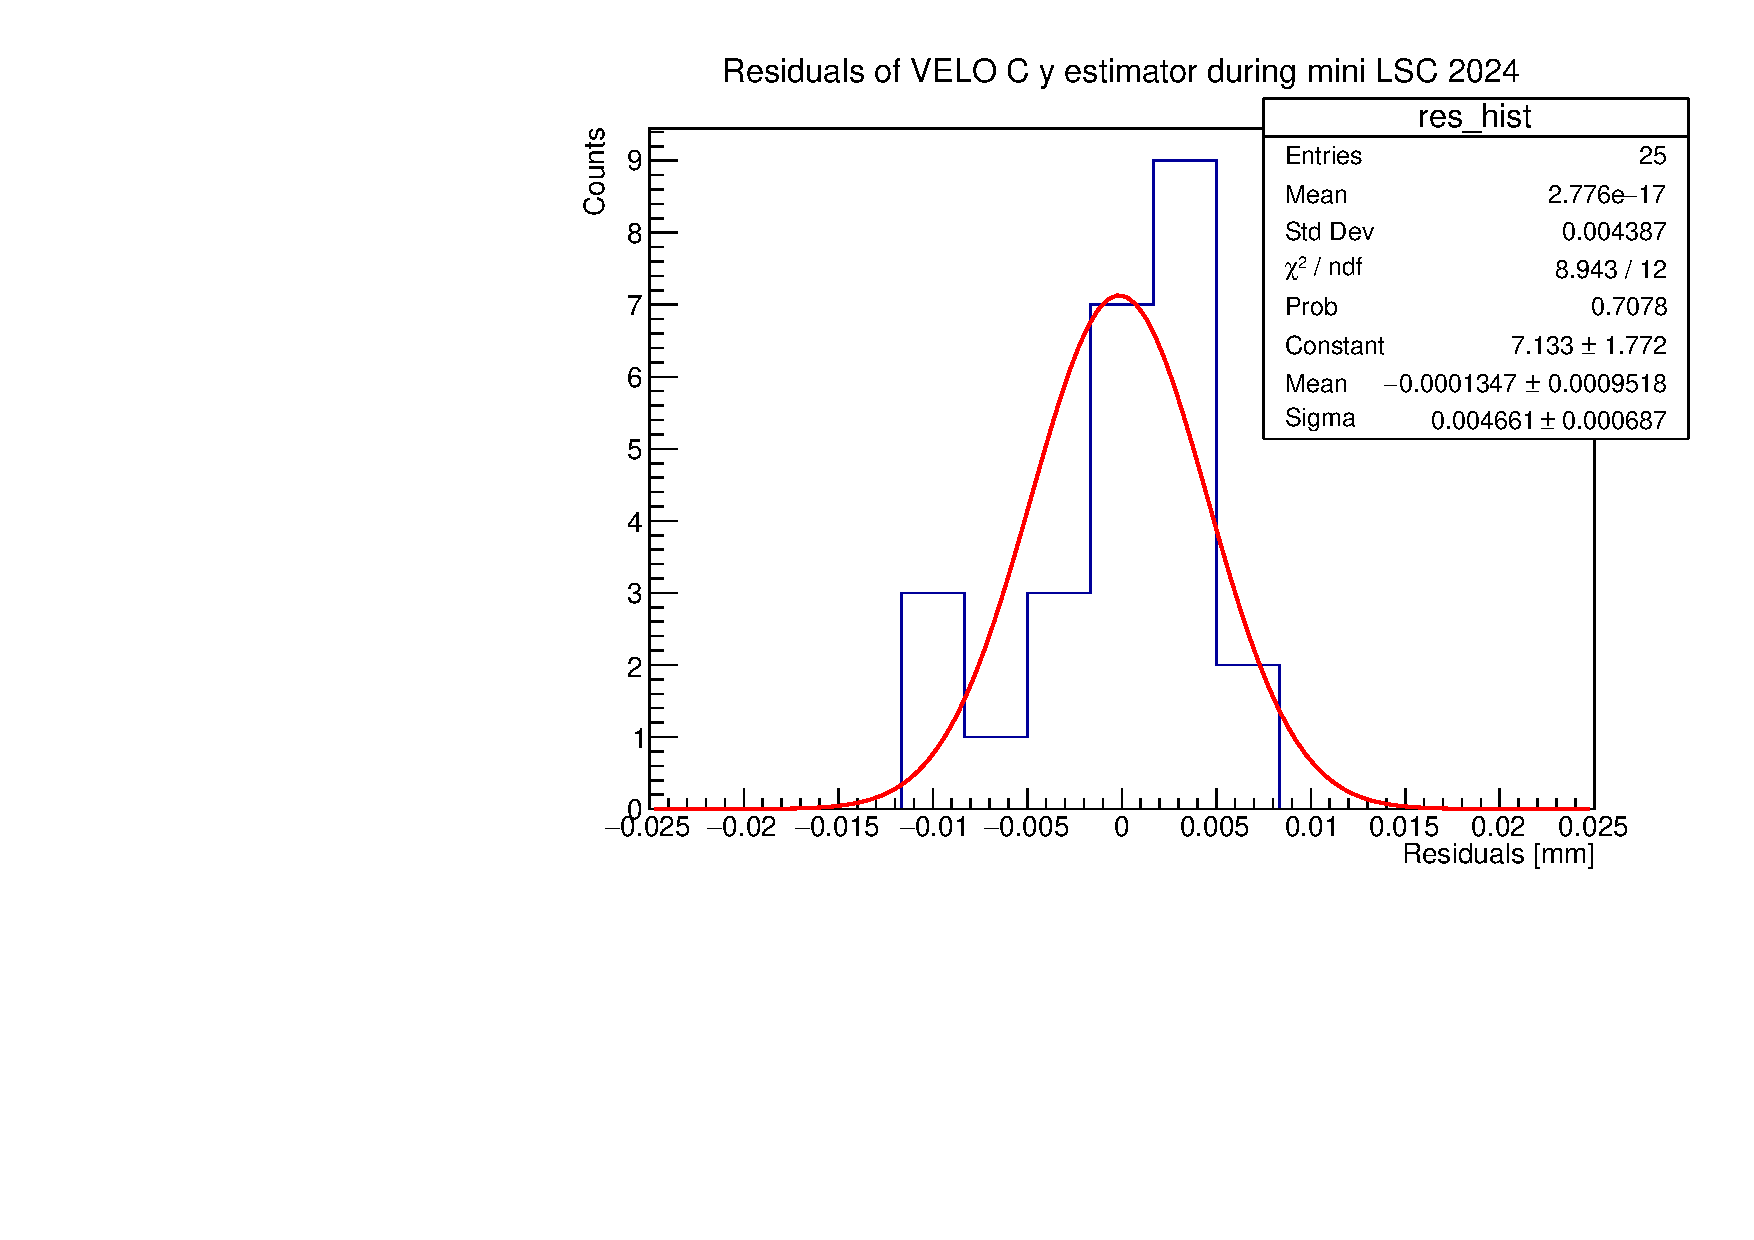
\includegraphics[width=\linewidth]{figures/y_res_VELO_C_data.pdf}
    \caption{Residuals from the fit of the graph on the left. }\label{fig:y_veloC_res_data}
    \end{subfigure}
    \caption{Linearity of the first component calculated with the PCA with respect to  virtual VELO C position shifts in $y$ component, alongside the residuals distribution fitted with a Gaussian probability density function.}
    \label{fig:y_veloC_data}
\end{figure}

The scatter plots alongside the residuals of the fitted linear function are reported in Figures \ref{fig:x_veloA_data}, \ref{fig:y_veloA_data}, \ref{fig:x_veloC_data}, \ref{fig:y_veloC_data}, respectively for $\hat{x}_A$, $\hat{y}_A$, $\hat{x}_C$, $\hat{y}_C$. As we can see from these scatter plots the relation is linear, and from these fits we can infer the other parameters that allows to calculate the estimators $\hat{x}_A$, $\hat{y}_A$, $\hat{x}_C$, $\hat{y}_C$. In order to deal with the problem of outliers and missing counters, we apply the same algorithm \ref{alg:beamline} described at the end of Chapter \ref{chap:beamline}. 

We can see a preliminary result of this calibration in Figure \ref{fig:traceplot_xy}, where we report the trace-plot of the estimators (blue and green) during the two LSC, compared with the position of the VELO halves estimated by the monitoring task (orange and red). The data used for the calibration are those of the first ramps in $x$ and $y$ (referring to Figure~\ref{fig:mini-vdm}), meaning that starting from 13:32 the calibration holds and estimators behave as expected. This behaviour is appreciated particularly during the second ramp that starts in the $x$ component around 13:47.

\begin{sidewaysfigure}
    \centering
    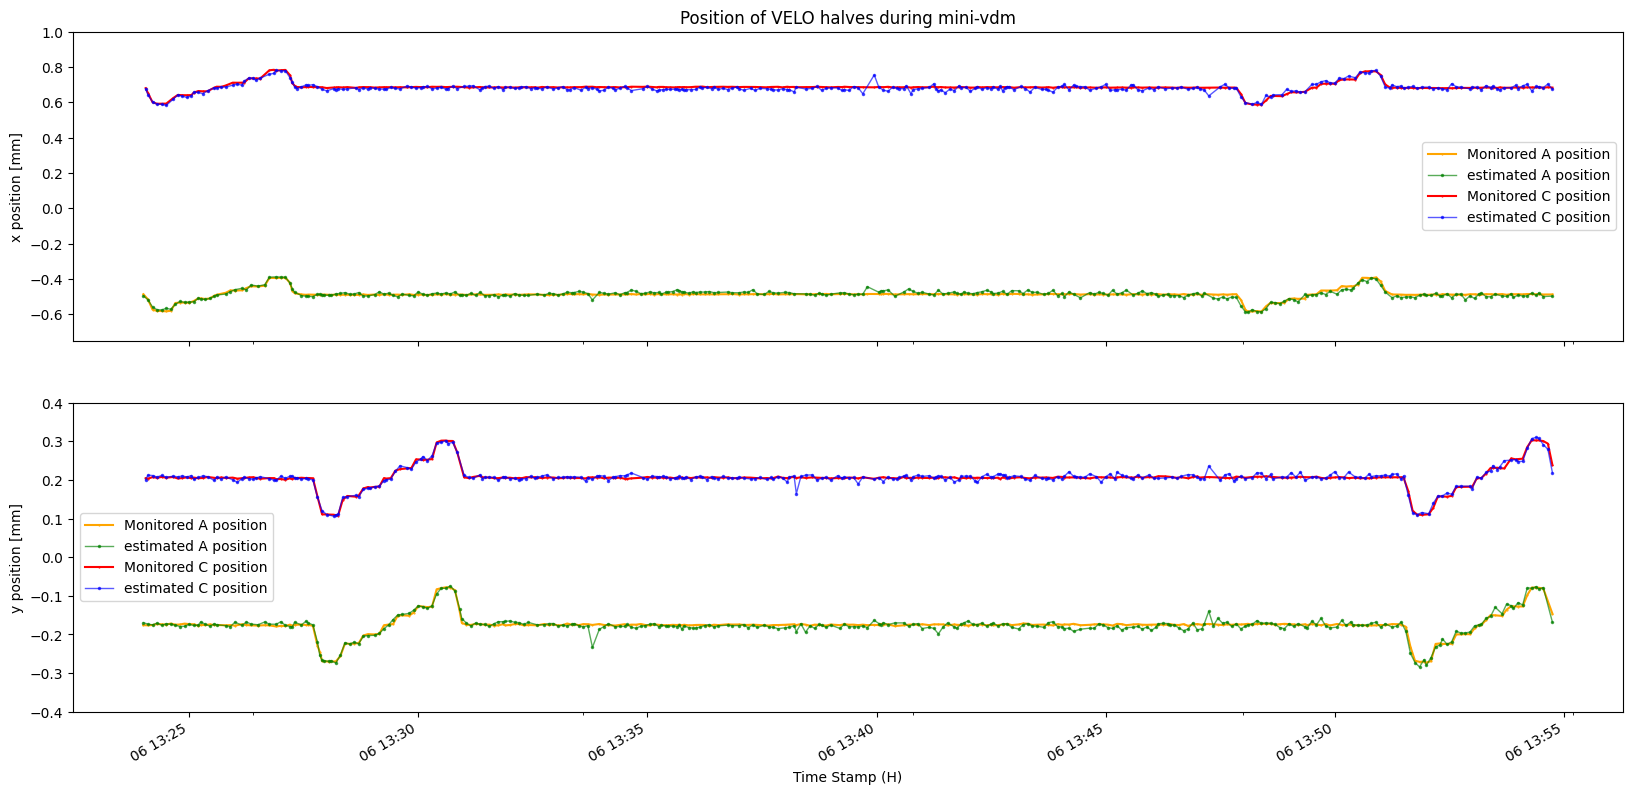
\includegraphics[width=\textwidth]{figures/traceplot_xy.png}
    \caption{Trace-plot of the VELO position estimators across the two VdM scans. In the upper panel, the $x$ position is displayed. The red and orange lines correspond to the monitored position of the two VELO halves, while the blue and the green ones to the estimated position presented in this chapter. An analogous situation is displayed in the second panel, for the $y$ position.}
    \label{fig:traceplot_xy}
\end{sidewaysfigure}

A more quantitative analysis of the correctness of the estimated positions $\hat{x}_A$, $\hat{y}_{A}$, $\hat{x}_C$, $\hat{y}_C$ can be performed by producing a scatter plot between the estimated positions and the positions provided by the monitoring tasks of the VELO. These scatter plots are produced using not only the region used in the calibration, but the whole fill. They are shown in Figures \ref{fig:xAfit_comparison}, \ref{fig:yAfit_comparison}, \ref{fig:xCfit_comparison}, \ref{fig:yCfit_comparison}, where on the left graph we performed a linear fit, while on the right we performed a Gaussian fit of the residuals. If there is complete agreement between these to quantities we expect the fitted angular coefficients to be $p_1=1$ and the offset $p_0=0$. 
The results of these fit are summarised in Table~\ref{tab:summary_velo}. There is good accordance between the coefficients, since they all differ 2.1 $\sigma$ or less from their expected values. 


\begin{figure}
    \centering
    \begin{subfigure}{0.48\textwidth}
    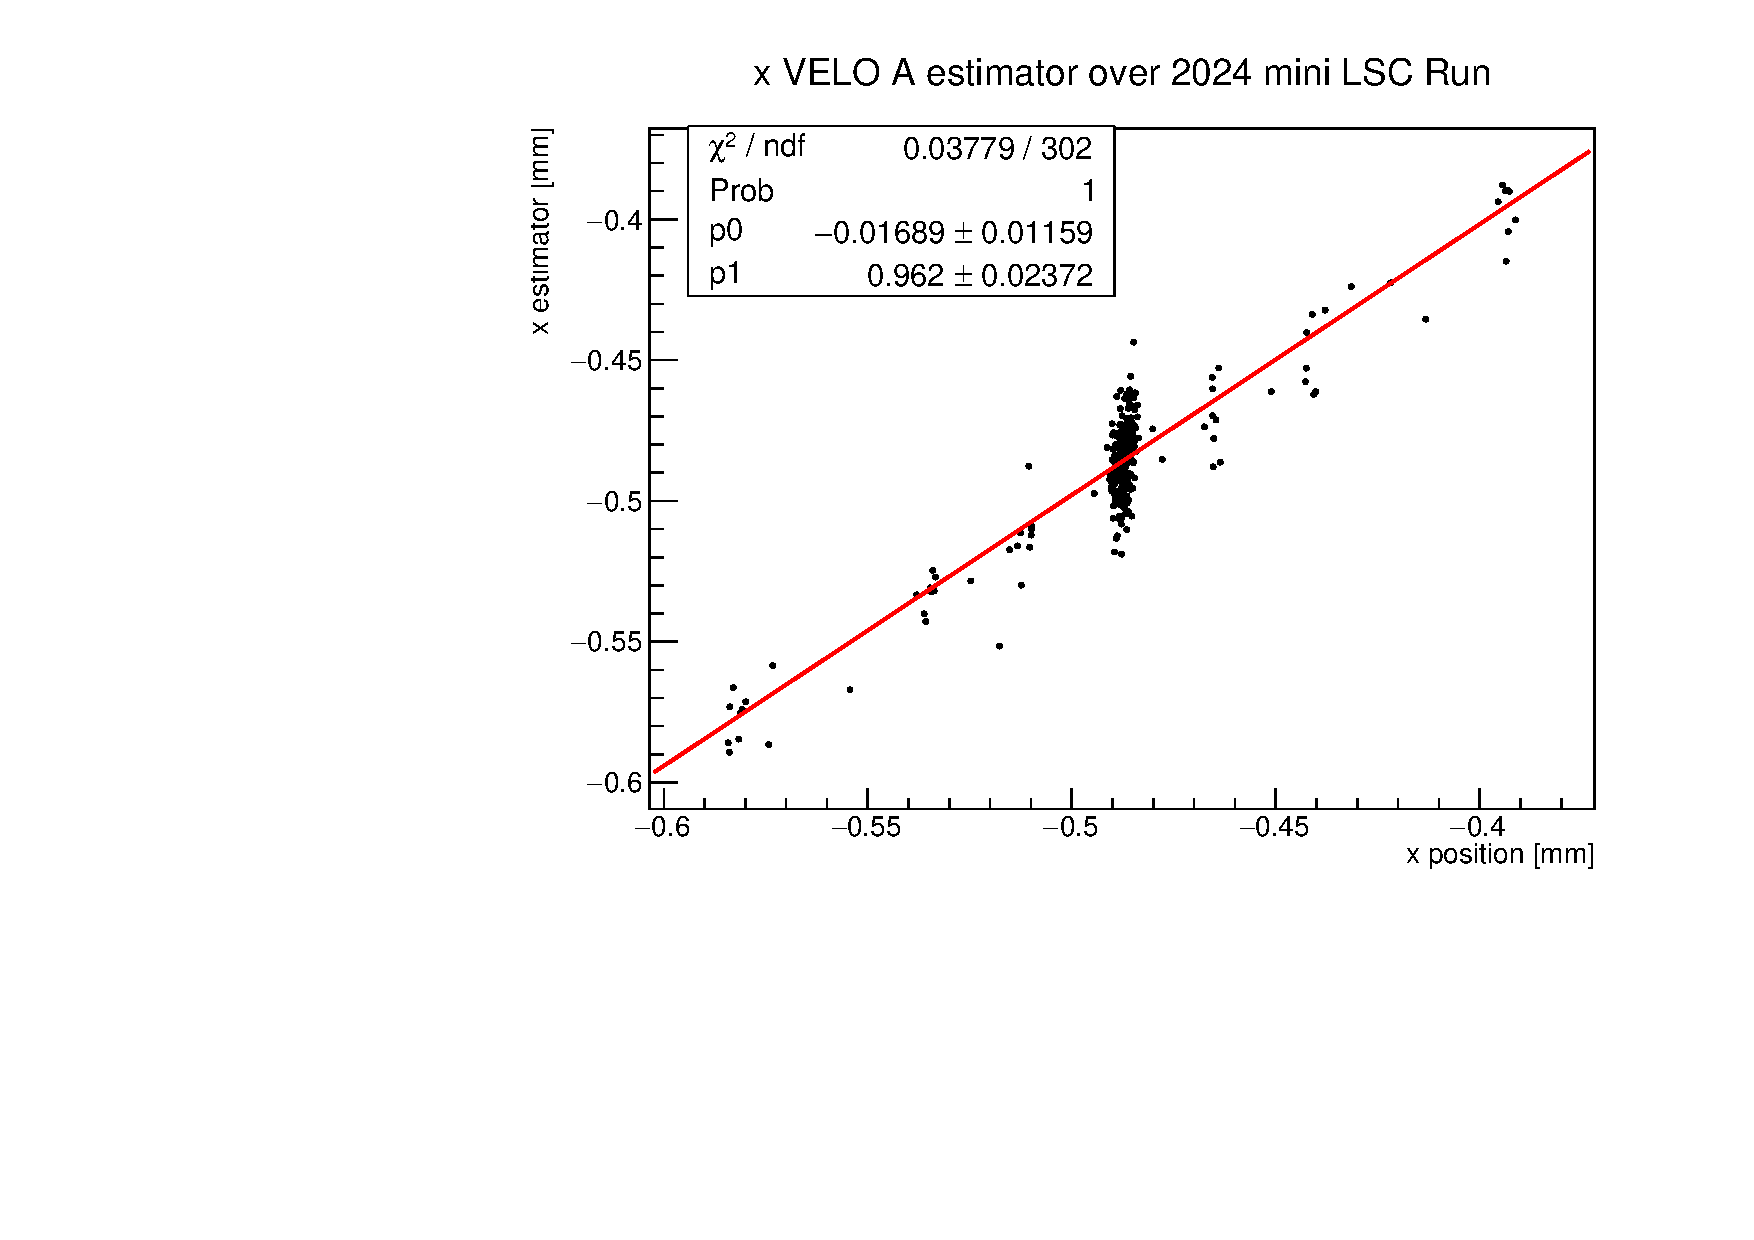
\includegraphics[width=\linewidth]{figures/xVeloA_fit_comparison.pdf}
    \caption{Linear Fit}\label{fig:xAfit_comparison}
    \end{subfigure}
    \begin{subfigure}{0.48\textwidth}
    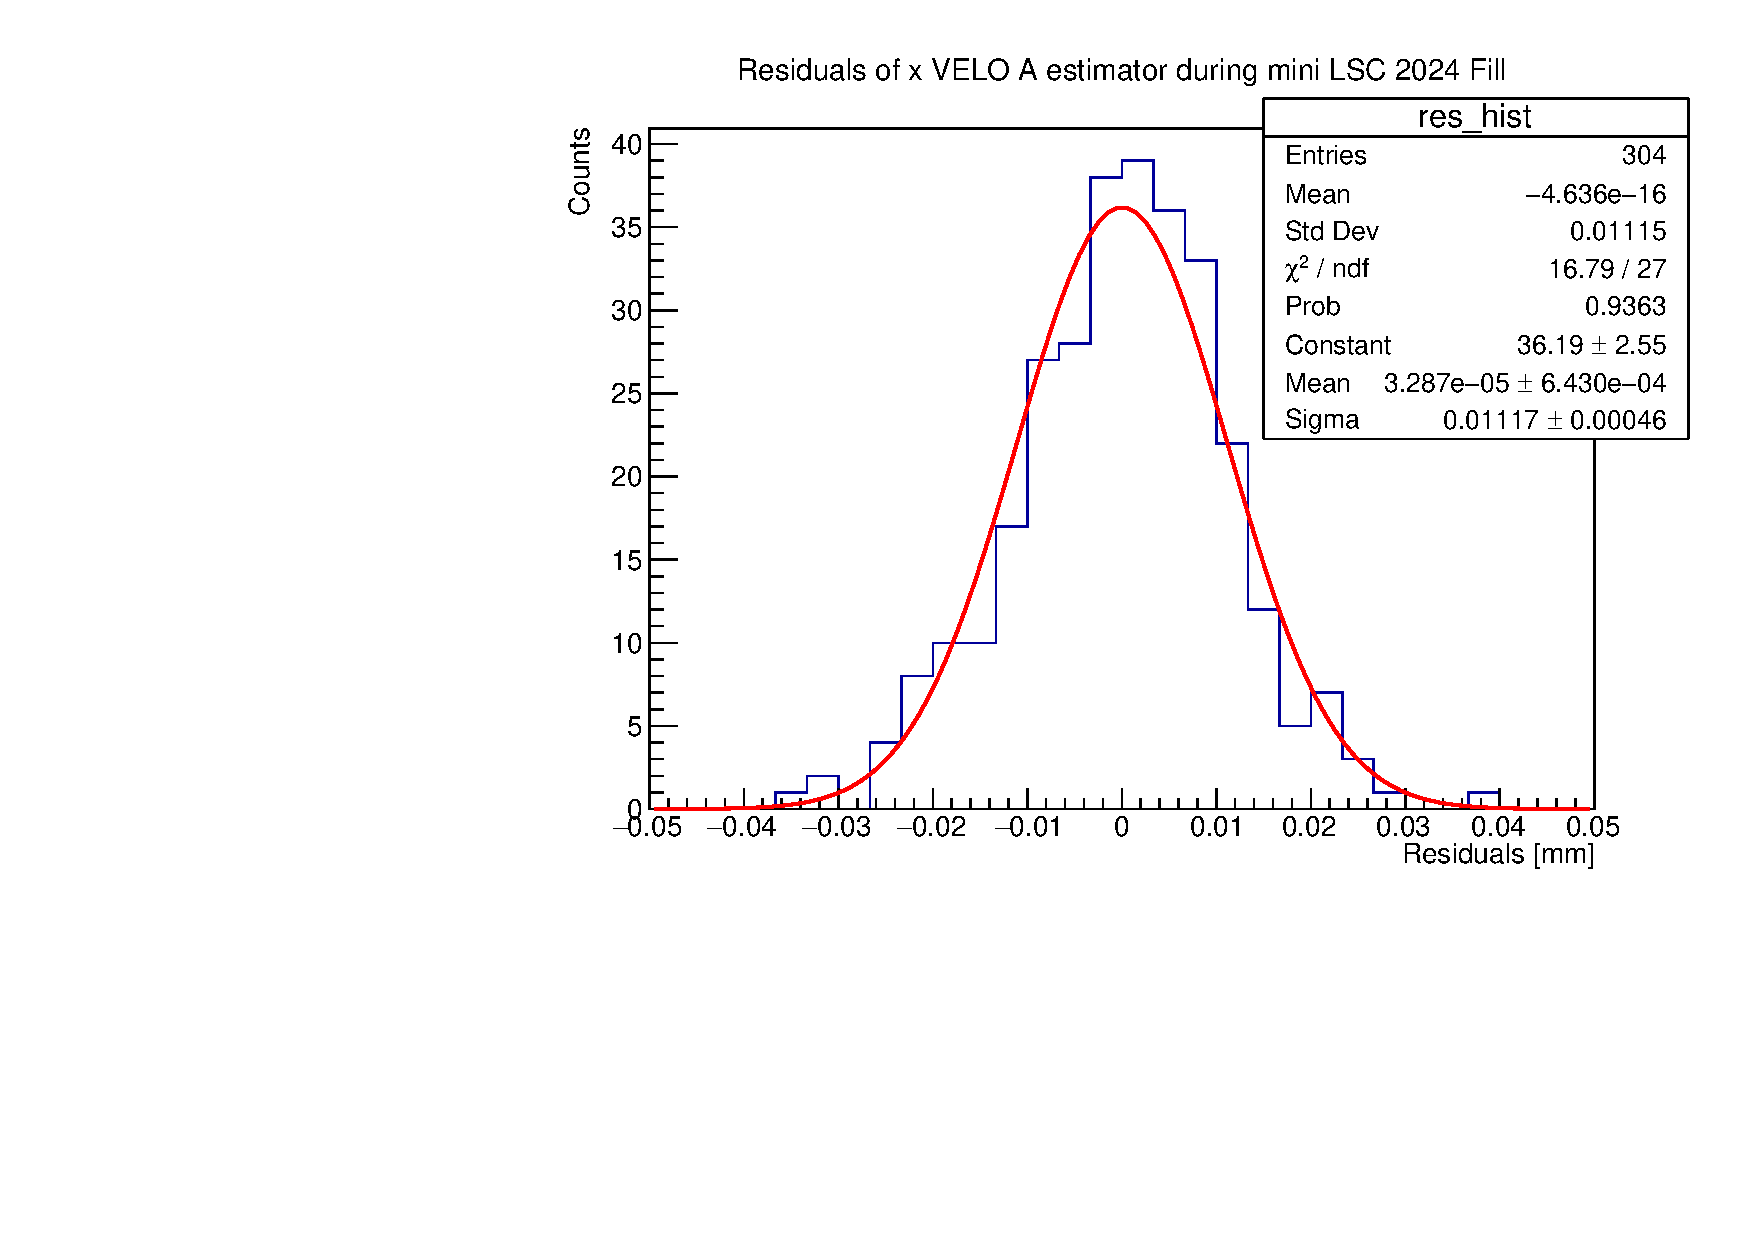
\includegraphics[width=\linewidth]{figures/xVeloA_res_compariosn.pdf}
    \caption{Residuals from the fit of the graph on the left. }\label{fig:xAres_comparison}
    \end{subfigure}
    \caption{$\hat{x}_{A}$ calibrated estimator vs monitored position shifts in $x$ component of the A side, alongside the residuals distribution fitted with a Gaussian distribution. The bulk in the centre of the scatter plot is due to the fact that our estimation is probably noiser than the one provided by the monitoring tasks. Having a lot of points for that particular position, the monitoring tasks provided measurements almost always in the same point, while our estimator as a wider distribution.}
    \label{fig:xA_comaprison}
\end{figure}
\begin{figure}
    \centering
    \begin{subfigure}{0.48\textwidth}
    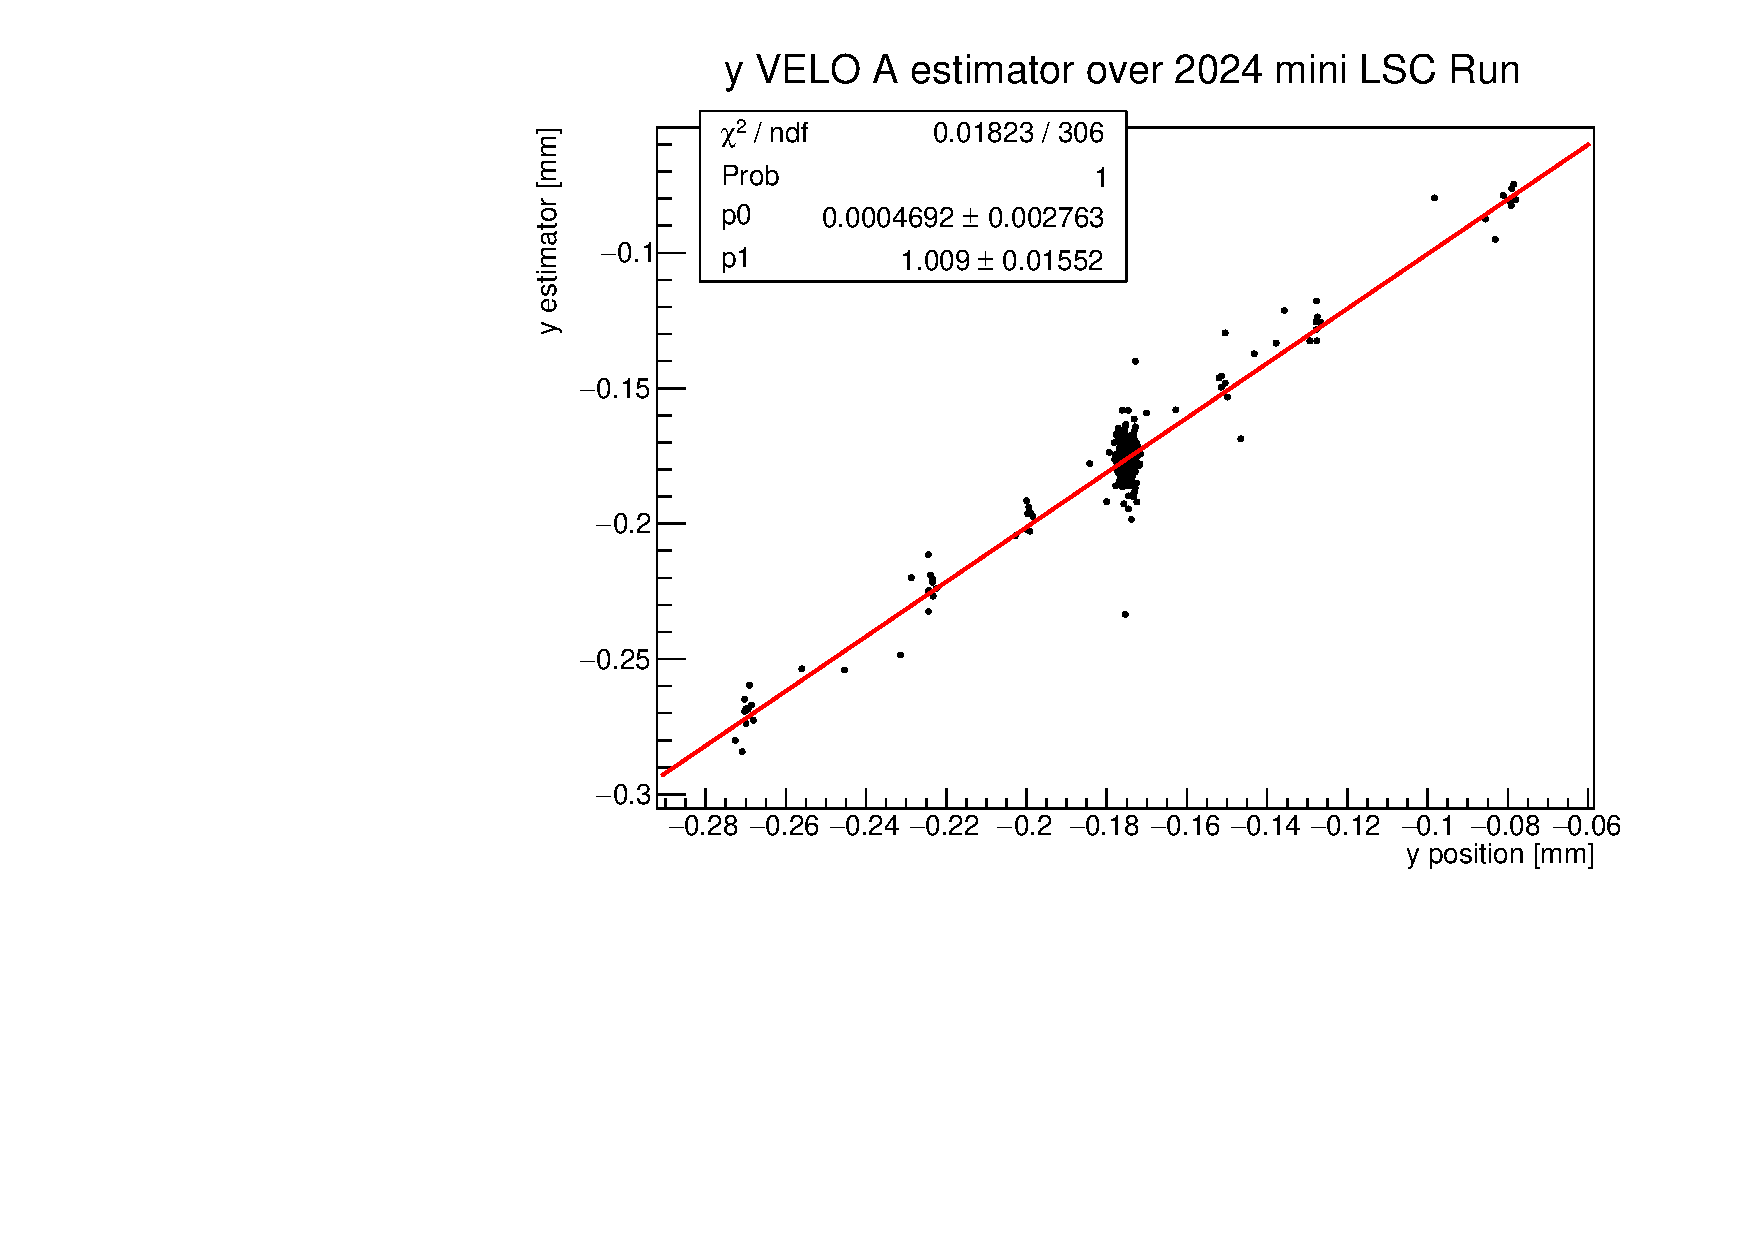
\includegraphics[width=\linewidth]{figures/yVeloA_fit_comparison.pdf}
    \caption{Linear Fit}\label{fig:yAfit_comparison}
    \end{subfigure}
    \begin{subfigure}{0.48\textwidth}
    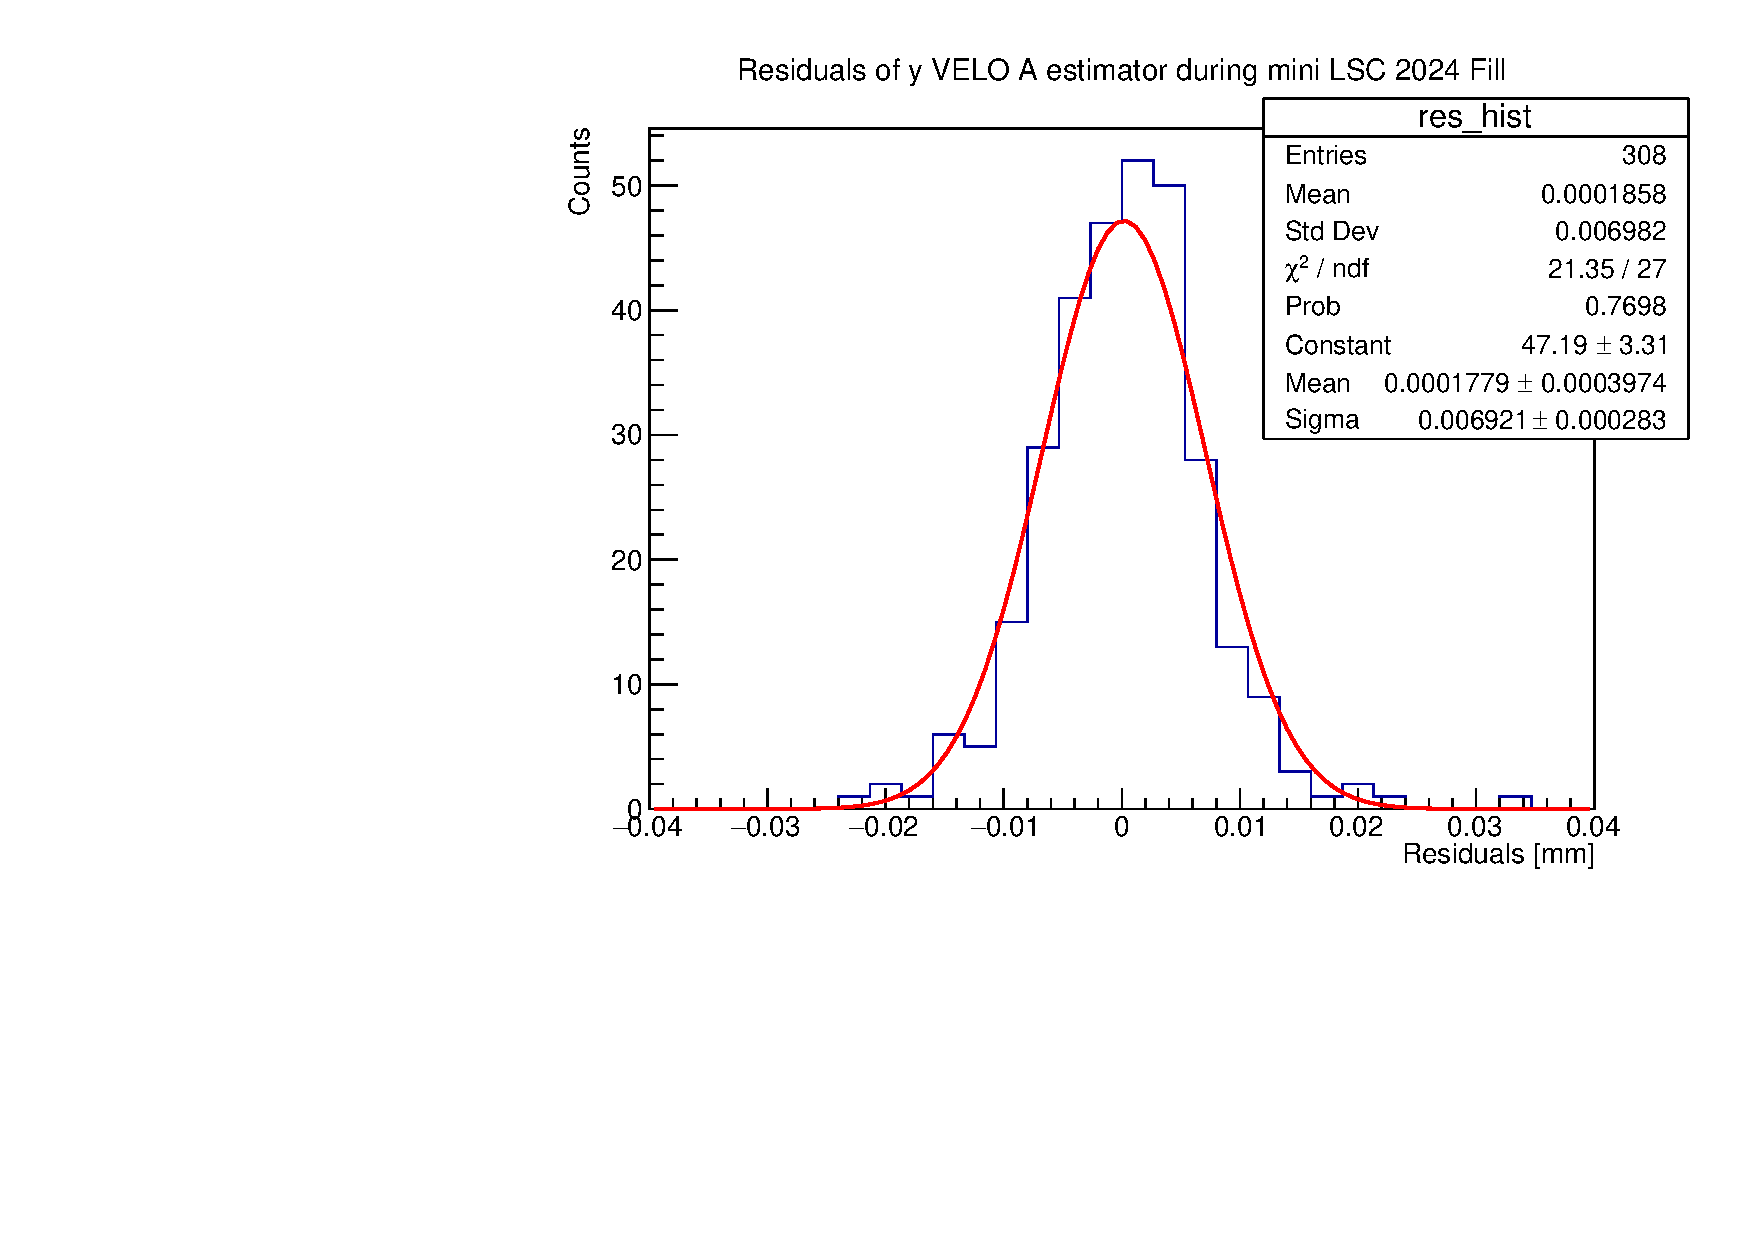
\includegraphics[width=\linewidth]{figures/yVeloA_res_comparison.pdf}
    \caption{Residuals from the fit of the graph on the left. }\label{fig:yAres_comparison}
    \end{subfigure}
    \caption{$\hat{y}_{A}$ calibrated estimator vs monitored position shifts in $y$ component of A side, alongside the residuals distribution fitted with a Gaussian distribution. The bulk in the centre of the scatter plot is due to the fact that there are a lot of point for that particular position. Our estimation is probably noiser than the one provided by the monitoring tasks. }
    \label{fig:yA_comparison}
\end{figure}

\begin{figure}
    \centering
    \begin{subfigure}{0.48\textwidth}
    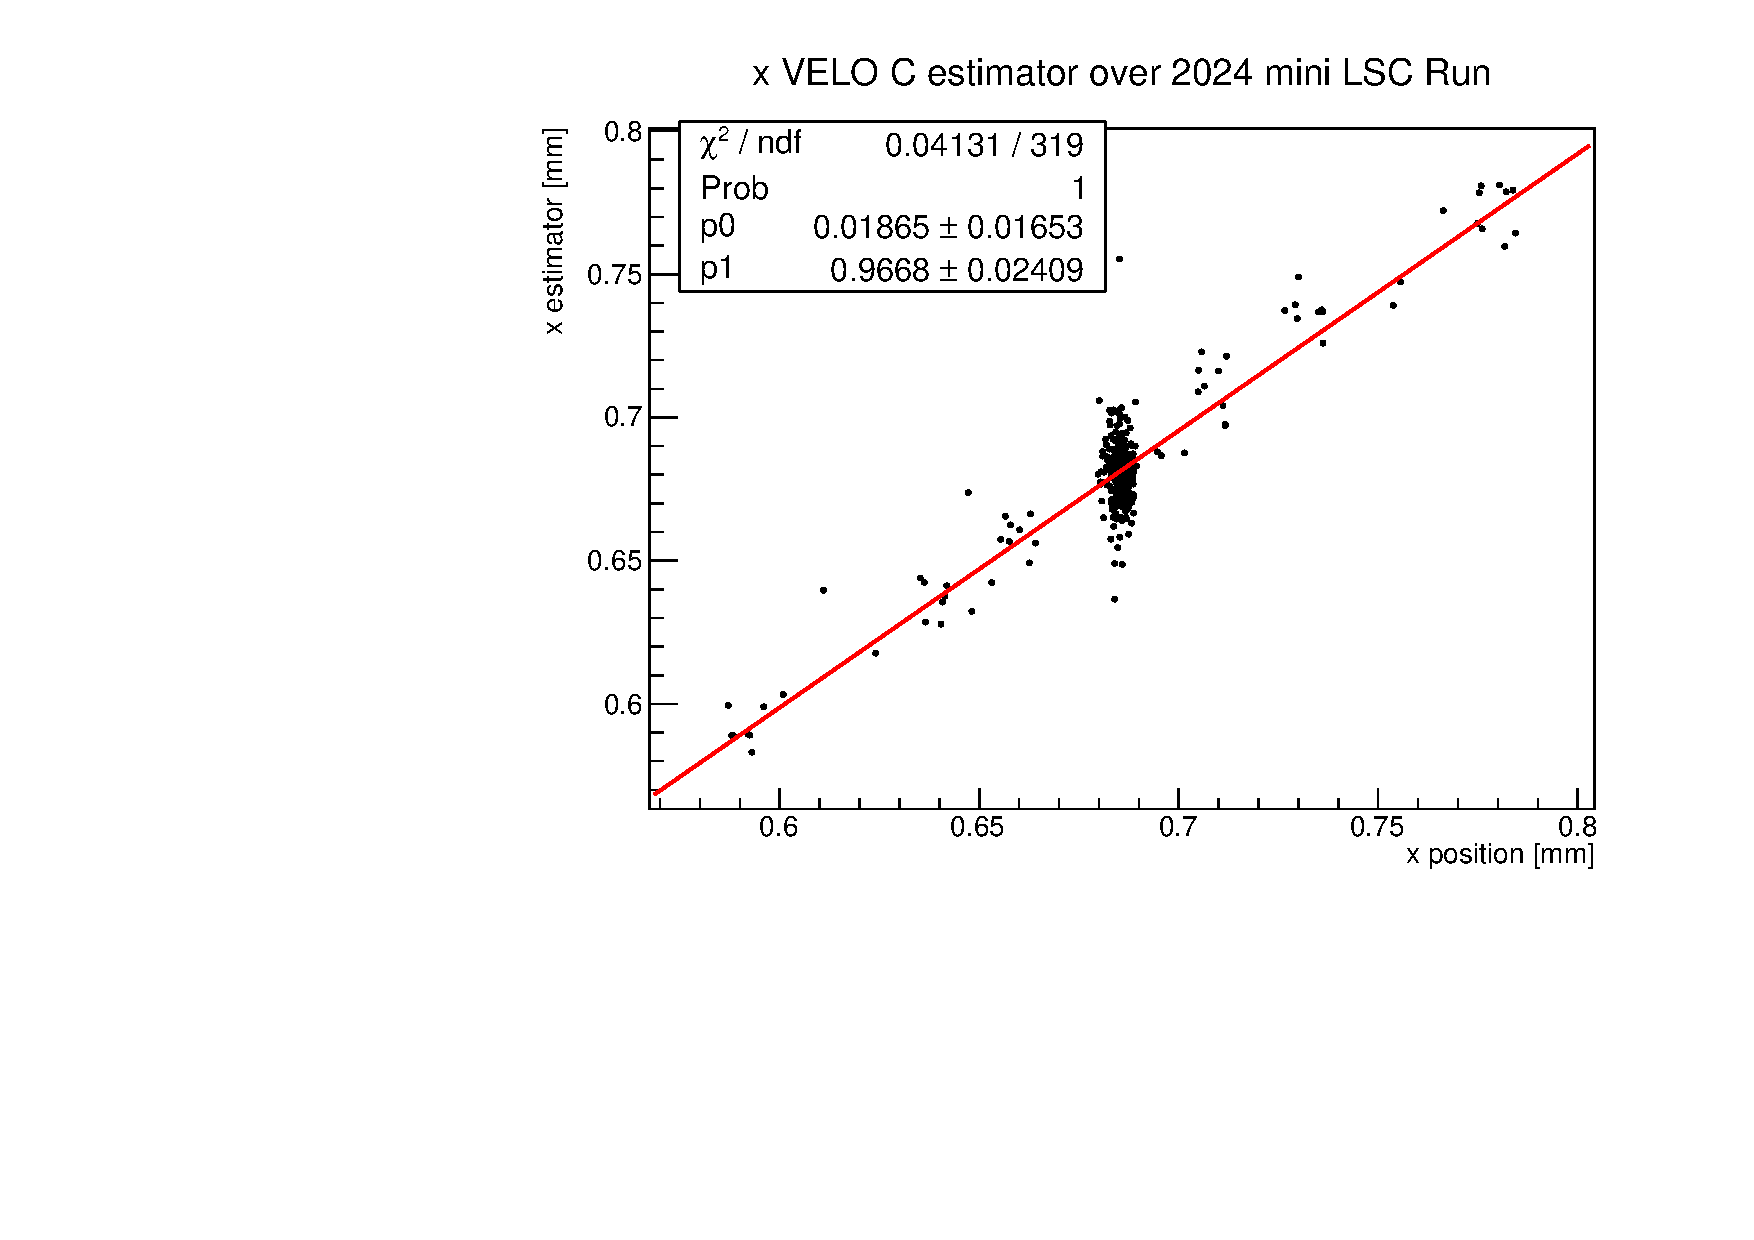
\includegraphics[width=\linewidth]{figures/xVeloC_fit_comparison.pdf}
    \caption{Linear Fit}\label{fig:xCfit_comparison}
    \end{subfigure}
    \begin{subfigure}{0.48\textwidth}
    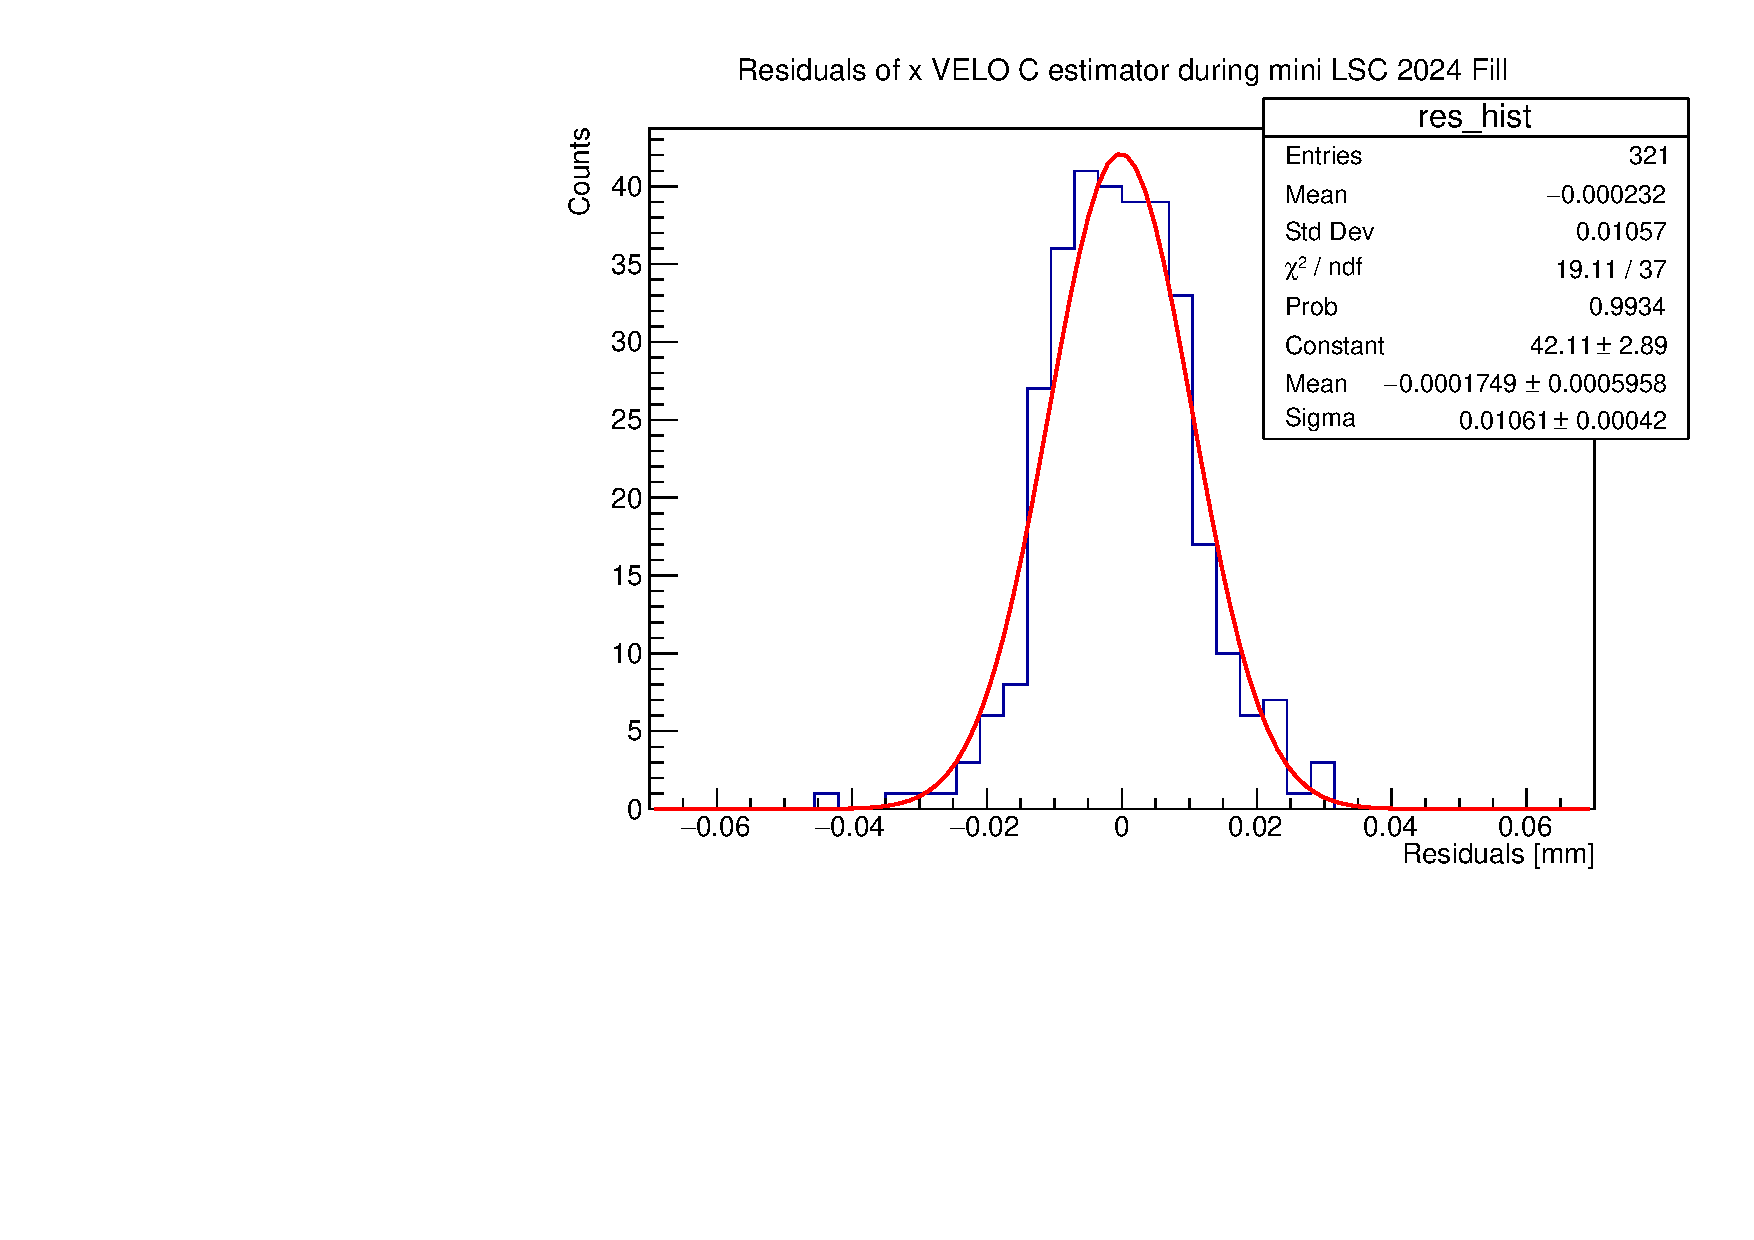
\includegraphics[width=\linewidth]{figures/xVeloC_res_comparison.pdf}
    \caption{Residuals from the fit of the graph on the left. }\label{fig:xCres_comparison}
    \end{subfigure}
    \caption{$\hat{x}_{C}$ calibrated estimator vs monitored position shifts in $x$ component of the C side, alongside the residuals distribution fitted with a Gaussian distribution. The bulk in the centre of the scatter plot is due to the fact that there are a lot of point for that particular position. Our estimation is probably noiser than the one provided by the monitoring tasks.}
    \label{fig:xC_comaprison}
\end{figure}
\begin{figure}
    \centering
    \begin{subfigure}{0.48\textwidth}
    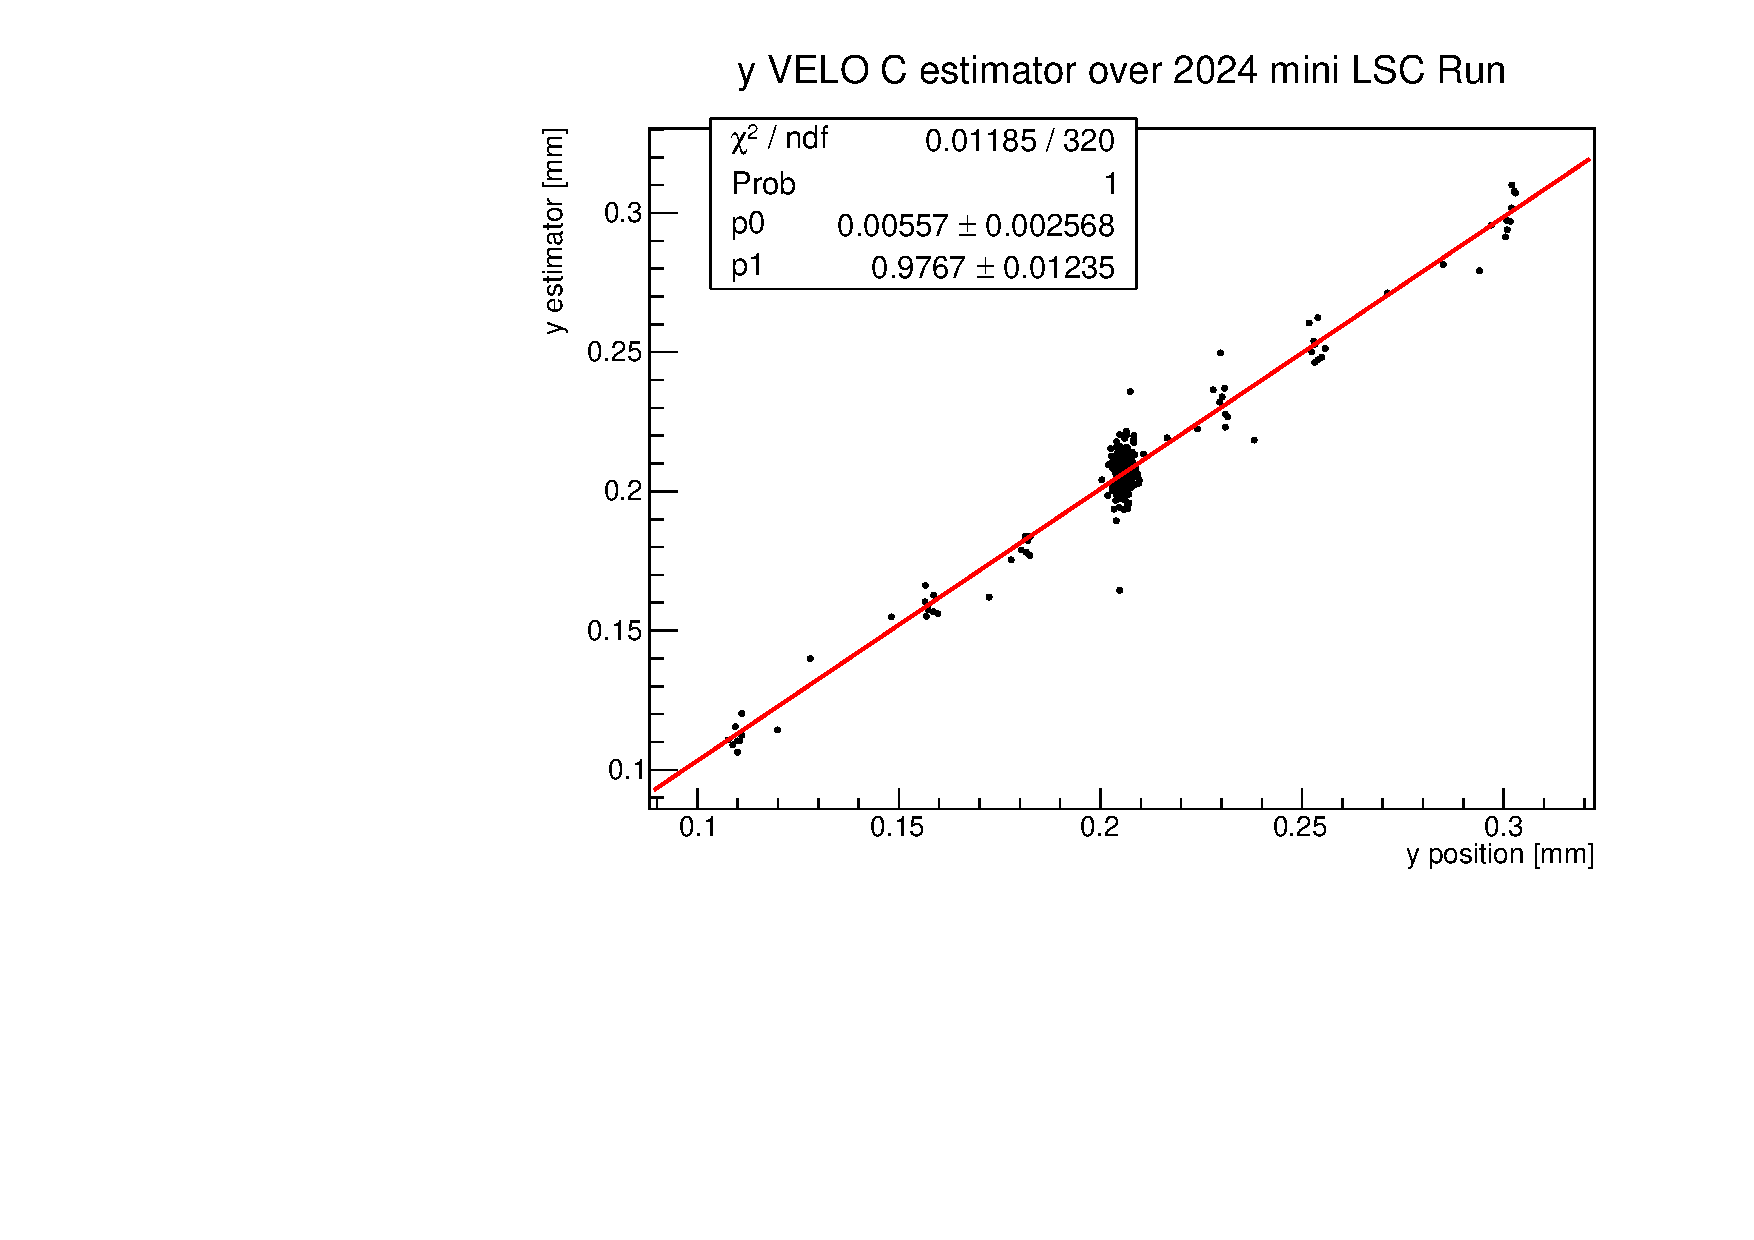
\includegraphics[width=\linewidth]{figures/yVeloC_fit_comparison.pdf}
    \caption{Linear Fit}\label{fig:yCfit_comparison}
    \end{subfigure}
    \begin{subfigure}{0.48\textwidth}
    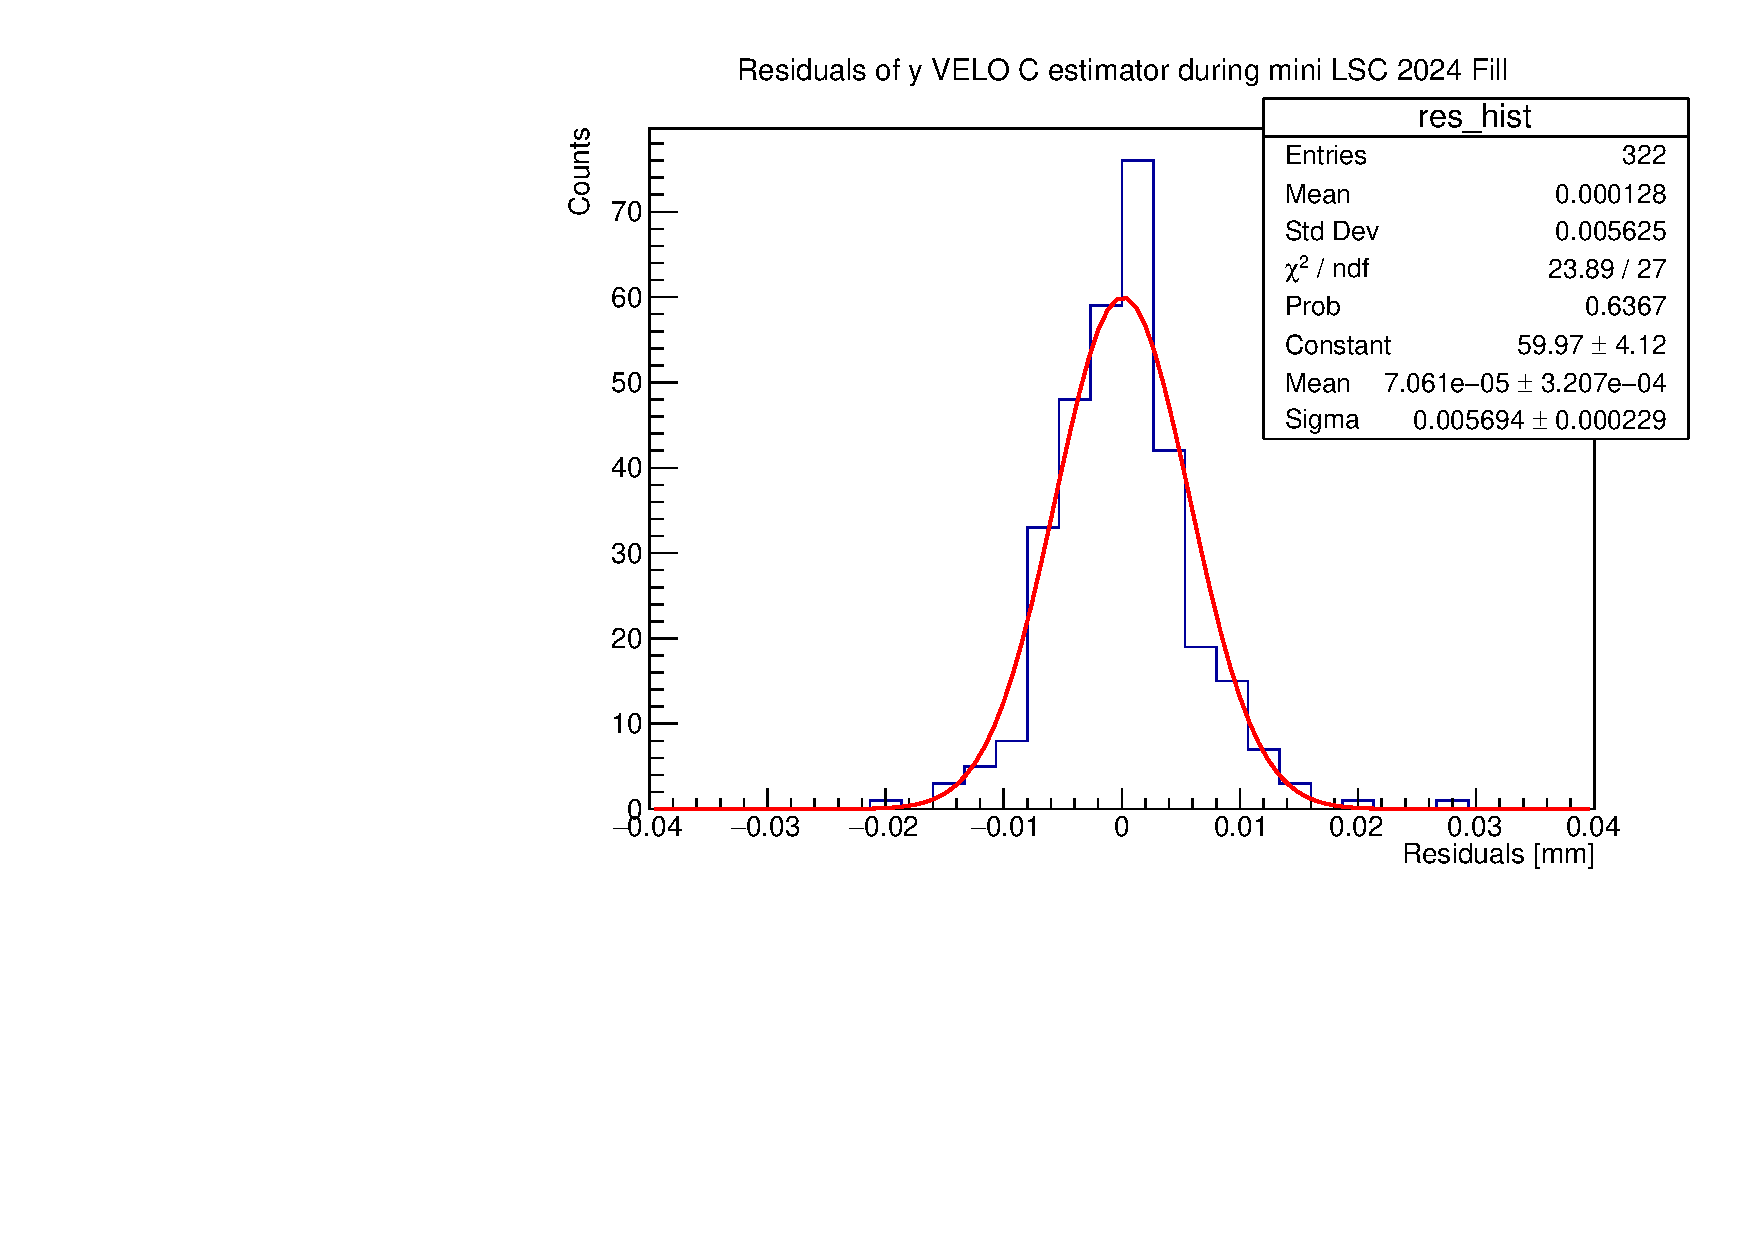
\includegraphics[width=\linewidth]{figures/yVeloC_res_comparison.pdf}
    \caption{Residuals from the fit of the graph on the left. }\label{fig:yCres_comparison}
    \end{subfigure}
    \caption{$\hat{y}_{C}$ calibrated estimator vs monitored position shifts in $y$ component of C side, alongside the residuals distribution fitted with a Gaussian distribution. The bulk in the centre of the scatter plot is due to the fact that our estimation is probably noiser than the one provided by the monitoring tasks. Having a lot of points for that particular position, the monitoring tasks provided measurements almost always in the same point, while our estimator as a wider distribution.}
    \label{fig:yC_comparison}
\end{figure}

\begin{table}
    \centering
    \begin{tabular}{c|c|c|c|c|c|c}
    variable  & $p_0$ & $p_1$ & $\sigma_{p_0}$ & $\sigma_{p_1}$ & $\Delta p_0$ [$\sigma$] & $\Delta p_1$ [$\sigma$]\\
    \hline
       $x_A$  & -0.017 & 0.962 & 0.011 & 0.024 & 1.5 & 1.6\\
       $y_A$  & 0.00047 & 1.009 & 0.0028 & 0.015 & 0.2 & 0.6 \\
       $x_C$ & 0.019 & 0.967 & 0.016 & 0.024 & 1.2 & 1.4\\
       $y_C$ & 0.0056 & 0.977 & 0.0026 & 0.012 & 2.1 & 1.9
    \end{tabular}
    \caption{Summary of the comparison between estimators and monitored positions by the VELO. The Deltas refer to the difference of the coefficients from their expected value $p_0=0$, $p_1=1$.}
    \label{tab:summary_velo}
\end{table}

Once the calibration performed on the data is validated, we can compare it to the calibration performed in Monte Carlo. As a comparison, we report in Table~\ref{tab:comparison_coeff} the estimated coefficients from both the Monte Carlo and the data, as well as the difference  between the two values expressed in units of the uncertainty $\sigma$ of the data-estimated parameters.

\begin{table}
\centering
\begin{tabular}{
c |
c |
c |
c |
c |
c |
c }
 & $a_{\text{MC}}$ & $a_{\text{data}}$ &  $\Delta a$ [$\sigma_a$] & $b_{\text{MC}}$ &  $b_{\text{data}}$ &  $\Delta b$ [$\sigma_b$] \\ \hline
    { $x_A$} &
  { $44.29$} &
  { $43.13\pm1.03$} &
  $1.12$ &%{ $2.7\%$} &
  { $-11.63$} &
  { $-11.91\pm0.27$} &
  $1.04$\\%{ $2.3\%$} \\
    { $x_C$} &
  { $-43.05$} &
  { $-46.62\pm1.26$} &
  $2.83$&%{ $7.6\% $} &
  { $11.99 $} &
  { $13.33\pm0.34$} &
  $3.94$\\%{ $10\%  $} \\
    { $y_A$} &
  { $-43.97$} &
  { $-55.46\pm 1.16$} &
  $9.90$ &%{ $26\%  $} &
  { $0.127 $} &
  { $-0.051\pm0.003$} &
  $59.33$\\%{ $349\% $} \\
    { $y_C$} &
  { $42.77 $} &
  { $43.91\pm0.80 $} &
  $1.41$&%{ $2.6\% $} &
  { $-0.155$} &
  { $0.123\pm0.002 $} &
  $139$%{ $226\% $}
\end{tabular}
\caption{Summary and comparison of coefficients estimated from MC and estimated from data. }\label{tab:comparison_coeff}
\end{table}
This comparison is of great use, as we can see that the calibration for the $x_A$ estimators are similar to one another, with the difference of the order of  $1\sigma$. As for the other estimators, there is strong disagreement with differences reaching $139\sigma$. An explanation for this disagreements could be given by the fact that the MC refers to 2022 conditions and the VELO was fully re-installed after 2023 YETS, thus introducing possible sizeable shifts and changes in detector efficiencies. 


%\section{A testing scenario: monitoring the VELO drift}
%\textit{Se ce la faccio, riporto il grafico del drift del VELO sovraimposto ai miei stimatori}

\section{Integration in the LHCb monitoring system}\label{sec:integration_detector}
As described in Section \ref{sec:beamline_integration}, the first step needed for the integration into the LHCb online system is the creation and deployment of the datapoints of the quantity estimated. This case is fully analogous to the one already described in Section~\ref{sec:beamline_integration}, therefore we just modified the WinCC script already written for the luminous region position estimators. The web page displaying the luminous region position is therefore updated adding the VELO halves position estimators in the same canvas of the luminous region estimators. As an example, we report in Figure \ref{fig:VELO_closing_xy} a screenshot of the $x$ and $y$ position canvases during the start of the Fill 9602 of May, 5th 2024. During the period displayed the closing procedure of the VELO was performed, and this is clearly visible in the upper panel where the two halves are shown to become closer as the time passes. Around 1:31 a second closing procedure is performed, therefore we see the VELO opening and closing once again along the $x$ component, as expected Adjustments in the $y$ component are also appreciable.
\begin{figure}
    \centering
    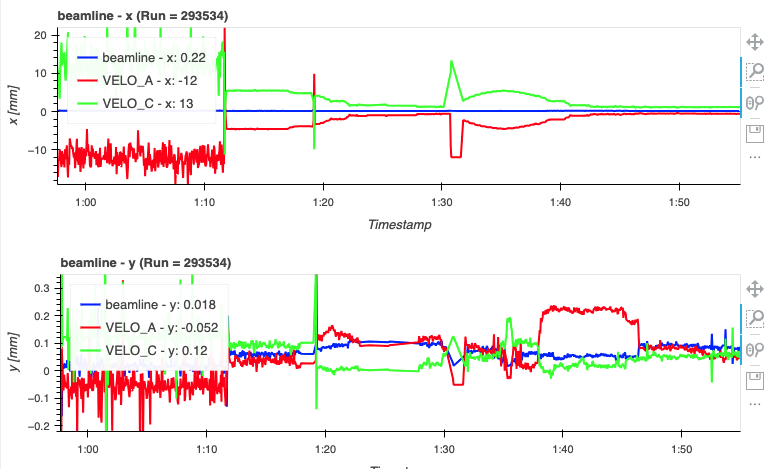
\includegraphics[width=\textwidth]{figures/VELO_closing_xy.png}
    \caption{Screenshot of the canvas in the Monet web page at the start of Fill 9602. The closing movements are evident, especially in the upper plot, where we can appreciate the two halves progressively moving towards 0. During this Fill, the closing procedure was performed twice, hence we see the VELO opening and closing again around 1:31. Adjustments in the $y$ component can also be appreciated.} 
    \label{fig:VELO_closing_xy}
\end{figure}

A zoom on the $x$ component estimators is reported in Figure \ref{zoom_velo}. In particular, in Figure \ref{fig:velo_closing_zoom} we see a zoom on the first closing procedure displayed in the upper panel of Figure \ref{fig:VELO_closing_xy}, while in Figure \ref{fig:velo_opens_zoom} we can clearly see the opening movements of the VELO at the end of Fill 9602.

\begin{figure}
    \centering
    \begin{subfigure}{0.8\textwidth}
    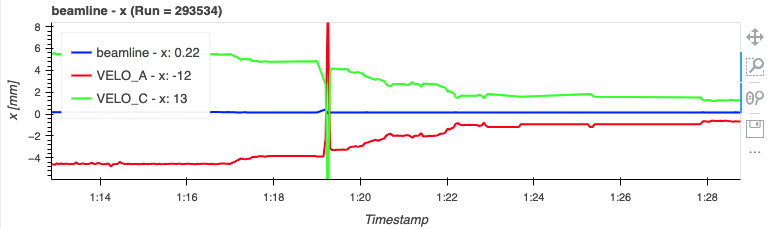
\includegraphics[width=\linewidth]{figures/Velo_closing_zoom.png}
    \caption{Zoom on the first VELO closing procedure of Fill 9602}
    \label{fig:velo_closing_zoom}
    \end{subfigure}\hfill
    \begin{subfigure}{0.8\textwidth}
    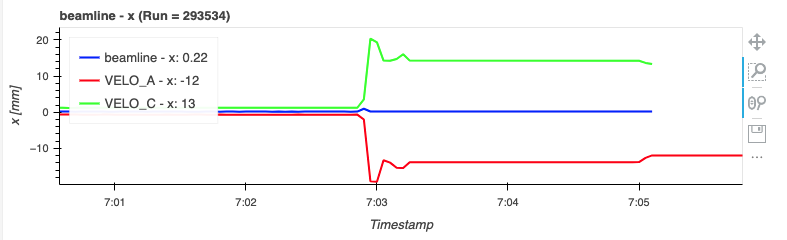
\includegraphics[width=\linewidth]{figures/VELO_opens_zoom.png}
    \caption{Zoom on the opening of the VELO at the end of Fill 9602}
    \label{fig:velo_opens_zoom}
    \end{subfigure}
    \caption{Zoom on two regions of the $x$ component estimators during the start and end of Fill 9602. The closing procedure is appreciated with greater detail in Figure \ref{fig:velo_closing_zoom}, respect to Figure \ref{fig:VELO_closing_xy}.}\label{zoom_velo}
\end{figure}
In Figure \ref{fig:fill9602} we report the behaviour of the estimators during the whole Fill 9602. As one can clearly see, both VELO halves in the $x$ component seem to be stable throughout the Run, except for a small drift of VELO A around 6:30. Regarding the $y$ component, the estimators sense shifts in both the luminous region position as well as the VELO C. In particular, at 4:00 a significant shift of $\sim\SI{30}{\micro\meter}$ in the position of the C side of the VELO is captured. Since the VELO A position in the $y$ component stays more or less constant in time (from 2:00 to 6:30), we can infer that the movement at 4:00 is in fact due to a shift of the C side of the VELO and not an artefact due to luminous region movements. The $y$ component of the luminous region (blue line) is shifted at 4:00 because its position is measured with respect to both VELO halves. Since one of them moved, its measured position changes. In the second panel of Figure \ref{fig:fill9602} we notice another movement around 6:30, due to a shift of the A side of the VELO.
\begin{figure}
    \centering
    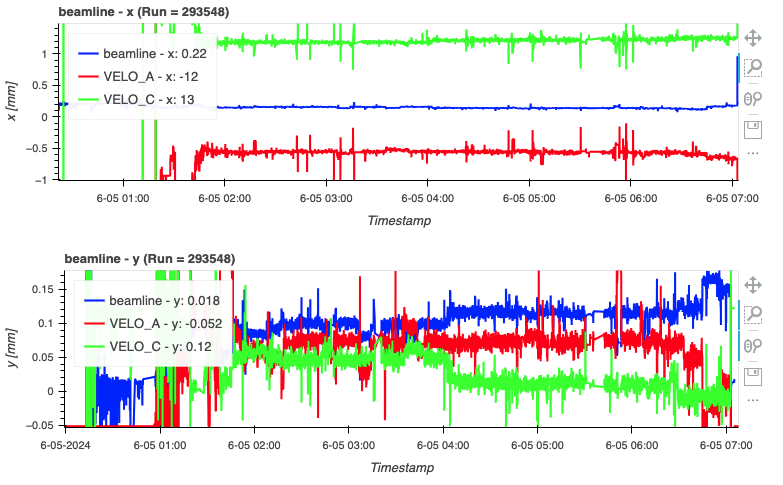
\includegraphics[width=\textwidth]{figures/Fill9602.png}
    \caption{Screenshot of the Monet web page comprehending the whole 9602 Fill}
    \label{fig:fill9602}
\end{figure}

These movements need to be confirmed by another monitoring task, but from these plots we can already appreciate how these estimators are of utter importance, sensing movements in real time. Furthermore, the shifts of $\sim\SI{30}{\micro\meter}$ are significant on the resolution scale of a single VELO measurement. 